% The search budget of the BSM resonance program.
%
% Public companion to the ATLAS-internal signal-catalogue note: everything here derives from
% published searches and public model databases, and is reproducible from this repository alone.
%
% Plain article + natbib so that it compiles anywhere.
\documentclass[11pt,a4paper]{article}

\usepackage[a4paper,margin=2.5cm,headheight=14pt]{geometry}
\usepackage{amsmath,amssymb}
\usepackage{graphicx}
\usepackage{booktabs}
\usepackage{array}
\usepackage{tabularx}
\usepackage{longtable}
\usepackage{xcolor}
\usepackage[font=small,labelfont=bf]{caption}
\usepackage{subcaption}
\usepackage{enumitem}
\usepackage{microtype}
\usepackage{fancyhdr}
\usepackage[numbers,sort&compress]{natbib}
\usepackage[colorlinks=true,linkcolor=blue!50!black,citecolor=blue!50!black,
            urlcolor=blue!50!black]{hyperref}

\graphicspath{{../../results/plots/}{../../results/plots/max_of_gaussians/}}

\newcommand{\code}[1]{\texttt{\small #1}}
\newcommand{\Nsig}{N_{\mathrm{trials}}}
\newcommand{\Zloc}{Z_{\mathrm{local}}}
\newcommand{\Zglob}{Z_{\mathrm{global}}}
\newcommand{\mtt}{m(t\bar{t})}
\newcommand{\GeV}{\ensuremath{\,\mathrm{GeV}}}
\newcommand{\TeV}{\ensuremath{\,\mathrm{TeV}}}
\newcommand{\fbinv}{\ensuremath{\,\mathrm{fb}^{-1}}}

\pagestyle{fancy}
\fancyhf{}
\fancyhead[R]{\small The search budget of the BSM resonance program}
\fancyfoot[C]{\thepage}
\renewcommand{\headrulewidth}{0.4pt}

\begin{document}

% ------------------------------------------------------------------ title page
\begin{titlepage}
\begin{center}
\vspace*{18mm}

{\LARGE\bfseries The search budget of the\\[2mm]
 BSM resonance program\par}
\vspace{8mm}
{\large How many independent bump hunts the model space implies,\\
 and what a discovery in that program costs\par}
\vspace{16mm}

{\large T.\ Reisch\par}
{\normalsize Universit\'e de Gen\`eve\par}
\vspace{4mm}
{\normalsize \today\par}
\vspace{18mm}

\begin{minipage}{0.86\textwidth}
\small
\textbf{Abstract.} Searches for new resonances are increasingly run as broad scans over many mass
spectra rather than as single model-specific measurements. For a scan of that kind the first number
one needs is not a limit but a count: how many independent looks does the program contain, and what
local significance does a discovery in it therefore have to reach? This note works that number out
from published information alone. Organising the public BSM resonance space by the spectrum in
which each model peaks, rather than by the theory that predicts it, collapses several dozen model
classes onto \textbf{46 distinct invariant- or transverse-mass spectra}, with lepton flavour and
$b$-tag content counted as part of the mass axis. Counting Gross--Vitells resolution elements over
the published scan window of each spectrum gives $\Nsig \approx 3.7\times10^{3}$ inclusively and
$6.6\times10^{3}$ at realistic event-selection granularity, so a $5\sigma$ global discovery costs a
local significance of $\Zloc \approx 6.4$ to $6.5$. That figure is stable to $\pm0.1\sigma$ against
every counting choice we varied, since the penalty enters only as $\ln \Nsig$, and the same
arithmetic reproduces the observed population of ATLAS excesses (tens at $3\sigma$, none spurious
at $5\sigma$). We then price a fully combinatorial scan ($\Nsig \approx 1.4\times10^{5}$, $\Zloc
\approx 7.0$), show that 57 of the 82 reachable object compositions have never been scanned by any
published ATLAS search, compare three candidate-selection rules on a common ROC, and evaluate a
two-stage A/B unblinding scheme that costs about $0.5\sigma$ in reach and buys an exactly countable
trials factor.
\end{minipage}
\end{center}
\end{titlepage}

\tableofcontents
\clearpage

\section{Introduction and scope}
\label{sec:intro}

\subsection{The question}

A conventional search fixes a model, a final state and a mass window before looking at data. The
look-elsewhere effect is then a modest correction applied at the end, and nobody worries much
about it. A growing fraction of the resonance program does not work that way. Model-independent
and data-directed scans~\cite{ddp}, machine-learning anomaly searches~\cite{atlas_ml_anomaly} and
general searches over many event classes~\cite{atlas_general_search} all sweep large parts of the
mass space at once, and for those the trials factor is not a footnote. It is the leading term in
what a discovery has to clear.

A prior question therefore needs a careful answer: how many independent looks does the BSM
resonance program actually contain? The number is usually quoted per analysis, if at all, and
never for the field as a whole. This note works it out from the ground up.

\begin{enumerate}[leftmargin=1.6em,itemsep=2pt]
  \item How many independent bump hunts does covering the public BSM model space imply, and what
        local significance does a $5\sigma$ global discovery therefore cost
        (Section~\ref{sec:budget})?
  \item What does the same arithmetic say about a fully combinatorial scan, and which object
        combinations has ATLAS in fact never scanned (Section~\ref{sec:combinatorial})?
  \item Is the resulting trials factor consistent with the excesses ATLAS has actually reported
        (Section~\ref{sec:excess})?
  \item Given a scan, how should candidates be selected: the largest bin, a threshold, or a
        false-discovery-rate rule (Section~\ref{sec:selection})?
  \item Does a two-stage A/B unblinding scheme make the trials factor cheaper, or only more
        defensible (Section~\ref{sec:ab})?
\end{enumerate}

\subsection{The one-paragraph answer}

The BSM resonance space looks unbounded at the level of models, with dozens of theories and
thousands of signal samples across them, and it collapses to \textbf{46 distinct invariant- or
transverse-mass spectra} once organised by where the bump appears, with lepton flavour and
$b$-tag content counted as part of the mass axis. Counting Gross--Vitells
resolution elements~\cite{grossvitells} over each spectrum's published scan window, the whole
program amounts to $\Nsig \approx 3.7\times10^{3}$ independent looks, rising to $6.6\times10^{3}$
when searches are sliced at realistic event-selection granularity. Because the penalty enters as
$\ln \Nsig$, that program costs a local bar of $\Zloc \approx 6.4$ to $6.5$ for a $5\sigma$ global
discovery, and the figure barely moves under any counting choice we varied. \textbf{Breadth is
cheap.} What is expensive is anything that makes $\Nsig$ uncountable, which is the situation a
neural-network-driven scan naturally creates, and the reason the two-stage unblinding discussion
in Section~\ref{sec:ab} matters even though splitting the data cannot reduce the look-elsewhere
effect.

\subsection{What this note does and does not use}

Every number here derives from two data-free ingredients: a curated list of bump observables with
their published scan windows, floors and resolutions (Appendix~\ref{app:windows}), and a map from
public BSM model classes to the spectra they populate. Both live in one module each in the
accompanying repository (Section~\ref{sec:software}), and neither reads a single experiment-internal
input --- no dataset identifiers, no signal-sample inventory, no unpublished analysis
configuration. Whether a given spectrum happens to have centrally produced Monte-Carlo samples
behind it is a question about a collaboration's production program rather than about the search
budget, and it is deliberately outside the scope of this note; a companion ATLAS-internal note
treats it.

One consequence is worth stating early, because it is what keeps the exercise
non-circular. Every spectrum is counted over the mass range a \emph{published} search family
scans, never over a range inferred from which signal samples exist. A search does not become
cheaper because few samples were generated for it.

\subsection{Conventions}

Throughout, one \emph{search} means one scanned mass spectrum, $n_s$ is the number of effective
independent resolution elements it contains, and $\Nsig = \sum_s n_s$. The local significance
required for a $5\sigma$ global discovery follows from
\begin{equation}
  \Zglob^2 \;=\; \Zloc^2 - 2\ln \Nsig
  \qquad\Longrightarrow\qquad
  \Zloc \;=\; \sqrt{25 + 2\ln \Nsig}\,,
  \label{eq:lee}
\end{equation}
the asymptotic Gross--Vitells relation~\cite{grossvitells} in the fixed-resolution-element
approximation. Masses are in GeV unless stated otherwise, and $\sqrt{s} = 13.6\TeV$.

Bibliographic details for the external searches quoted throughout were checked against the arXiv
metadata records and INSPIRE in August 2026.

\section{The search budget}
\label{sec:budget}

\subsection{Method}

One bump hunt is one scanned mass spectrum. For a spectrum with constant fractional mass resolution
$\sigma_M = r\,M$, the number of effectively independent resolution elements across a scanned
window $[M_{\mathrm{lo}}, M_{\mathrm{hi}}]$ is
\begin{equation}
  n_s \;=\; \frac{1}{r}\,\ln\!\frac{M_{\mathrm{hi}}}{M_{\mathrm{lo}}}\,,
  \label{eq:ns}
\end{equation}
summed over disjoint segments where a scan is not contiguous. The program's trials factor is
$\Nsig = \sum_s n_s$ and the discovery bar follows from Eq.~\eqref{eq:lee}. This is the
fixed-resolution-element form of the Gross--Vitells estimate~\cite{grossvitells}; the up-crossing
refinement adds a mild $Z$-dependence that is immaterial at the precision quoted here.

The fractional resolution $r$ is the only genuine physics input, so every headline is quoted with
a band obtained by varying $r$ by a factor two in each direction, which moves $\Nsig$ by a factor
two the other way.

\paragraph{The window convention, and why it matters.} Which range counts as ``scanned'' is the
one choice that can quietly bias the whole exercise. We count every spectrum over its
\textbf{published-search scan window}, meaning the mass range a real, published ATLAS search
family scans on that axis, extended where that family's published signal grid demonstrably
prepares a wider scan. Each window carries a per-channel source note
(Appendix~\ref{app:windows}).

The tempting alternative --- taking the range over which signal samples happen to have been
generated --- is wrong twice over. It understates sparsely sampled channels, since a search does
not become cheaper because few samples were made for it, and it ties a supposedly model-space
quantity to one collaboration's production choices. With the published-window convention the
budget is a statement about the searches the field has defined.

\paragraph{Scope.} Only invariant- and transverse-mass bump hunts enter the sum. The dedicated
non-bump programs, meaning displaced HNL, $Z_d$, RPV and ALP searches, MET$+$jet, $dE/dx$ monopole
and off-shell EFT, carry their own look-elsewhere effect and are not mass scans. They are excluded
rather than summed.

\paragraph{What counts as one spectrum.} Models are grouped by the mass axis in which they peak,
and two properties that a real analysis must select on are treated as part of that axis rather than
as cuts within it: \textbf{lepton flavour} and \textbf{$b$-tag content}. So $m(ee)$ and
$m(\mu\mu)$, and likewise $m(eb)$ and $m(ej)$, are separate spectra, each with its own resolution
and scan window. The justification is physical rather than bookkeeping: an electron pair is
measured in the electromagnetic calorimeter ($r \approx 0.015$, nearly mass-independent) while a
muon pair is measured by track sagitta ($r$ rising to $\sim$15\,\% at $3\TeV$, entered as a
window-averaged $r \approx 0.05$), and the two are scanned by separate analyses with separate
triggers. At low mass the ordering reverses, which is why the dark-photon electron channel starts
at $1\GeV$ and the muon channel at $0.3\GeV$. Because flavour is an axis here, it is \emph{not}
also counted in the event-selection multiplicities below; doing both would double-count it.

Conversely, decay modes that resolve onto the \emph{same} mass axis are merged: $X \to HH$ observed
in $4b$ is not a different spectrum from $X \to HH$, it is a different event selection of it, and it
is counted as such in Table~\ref{tab:granularity}.

\subsection{Result}

Table~\ref{tab:budget} gives the per-spectrum breakdown and Table~\ref{tab:budget_summary} the
totals. Covering every bump channel that public BSM models motivate costs
\begin{equation*}
  \Nsig = 3\,694 \quad\text{over 46 spectra}
  \qquad\Longrightarrow\qquad
  \Zloc = 6.44 \ \text{for a } 5\sigma \text{ global discovery.}
\end{equation*}
Equivalently, a local $5\sigma$ anywhere in that program is worth about $3\sigma$ globally.

\begin{table}[htbp]
\centering
\small
\caption{Trials per spectrum. $r$ is the assumed fractional mass resolution, the window is the
published-search scan range (Appendix~\ref{app:windows}) and $n_s$ follows from
Eq.~\eqref{eq:ns}. ``envelope'' is the reference count over the full kinematically accessible
range (analyzable floor to $\sqrt{s}$), ``\#mod'' the number of public model classes that predict a
peak in the spectrum, and ``\#sel'' the number of distinct published event selections that scan it
(Table~\ref{tab:granularity}).}
\label{tab:budget}
\begin{tabular}{rlcrrrrrr}
\toprule
\# & spectrum & $r$ & window [GeV] & $n_s$ & envelope & \#mod & \#sel & $n_s\times$sel \\
\midrule
1 & $m(\gamma\gamma)$ & 0.01 & 60--110 $+$ 150--5000 & 411 & 583 & 5 & 2 & 822\\
2 & $m(\mu\mu)$ ($Z_d$) & 0.02 & 0.3--400 & 360 & 536 & 2 & 1 & 360\\
3 & $m(ee)$ & 0.015 & 150--8000 & 265 & 321 & 7 & 1 & 265\\
4 & $m(ee)$ ($Z_d$) & 0.025 & 1--400 & 240 & 381 & 1 & 1 & 240\\
5 & $m(e\gamma)$ & 0.015 & 200--5000 & 215 & 328 & 1 & 1 & 215\\
6 & $m(e\mu)$ LFV & 0.03 & 100--8000 & 146 & 234 & 4 & 1 & 146\\
7 & $m(e^\pm e^\pm)$ SS & 0.015 & 200--1300 & 125 & 454 & 2 & 1 & 125\\
8 & $m(V\gamma)$ & 0.03 & 220--6000 & 110 & 141 & 3 & 2 & 220\\
9 & $m(ej)$ & 0.03 & 200--5000 & 107 & 234 & 3 & 4 & 429\\
10 & $m(\mu\gamma)$ & 0.03 & 200--5000 & 107 & 164 & 1 & 1 & 107\\
11 & $m(\mu j)$ & 0.04 & 200--5000 & 80 & 176 & 3 & 4 & 322\\
12 & $m(eZ)$ & 0.03 & 100--1100 & 80 & 164 & 1 & 1 & 80\\
13 & $m(\mu\mu)$ & 0.05 & 150--8000 & 80 & 96 & 7 & 1 & 80\\
14 & $m(cb)$ dijet & 0.05 & 20--1000 & 78 & 136 & 1 & 2 & 156\\
15 & $m(e^\pm\mu^\pm)$ SS & 0.025 & 200--1300 & 75 & 272 & 2 & 1 & 75\\
16 & $m(jj)$ & 0.05 & 200--8000 & 74 & 84 & 8 & 2 & 148\\
17 & $m(j\gamma)$ & 0.04 & 500--7000 & 66 & 113 & 2 & 1 & 66\\
18 & $m(\mu Z)$ & 0.04 & 100--1100 & 60 & 123 & 1 & 1 & 60\\
19 & $m(eb)$ & 0.04 & 200--2000 & 58 & 170 & 3 & 2 & 115\\
20 & $m(eejj)$ & 0.05 & 400--7000 & 57 & 76 & 2 & 1 & 57\\
21 & $m(VV)$ & 0.06 & 200--6000 & 57 & 74 & 12 & 9 & 510\\
22 & $m(bj)$ & 0.06 & 200--6000 & 57 & 70 & 1 & 2 & 113\\
23 & $m(Vh)$ & 0.06 & 200--5000 & 54 & 70 & 2 & 6 & 322\\
24 & $m(\mu^\pm\mu^\pm)$ SS & 0.04 & 200--1300 & 47 & 170 & 2 & 1 & 47\\
25 & $m(\mu b)$ & 0.05 & 200--2000 & 46 & 136 & 3 & 2 & 92\\
26 & multilepton & 0.12 & 50--10000 & 44 & 62 & 3 & 4 & 177\\
27 & $m(3j)$ & 0.05 & 200--1800 & 44 & 84 & 2 & 1 & 44\\
28 & $m(tb)$ & 0.08 & 180--6000 & 44 & 54 & 3 & 3 & 132\\
29 & $m(\tau\tau)$ & 0.12 & 35--6000 & 43 & 50 & 4 & 3 & 129\\
30 & $m(\mu\mu jj)$ & 0.07 & 400--7000 & 41 & 54 & 2 & 1 & 41\\
31 & $m(bb)$ & 0.1 & 15--62 $+$ 450--6000 & 40 & 68 & 4 & 3 & 120\\
32 & $m(HH)$ & 0.08 & 250--6000 & 40 & 50 & 4 & 6 & 238\\
33 & $m_{\mathrm{T}}(e\nu)$ & 0.1 & 150--7000 & 38 & 60 & 2 & 1 & 38\\
34 & $m(t\bar t)$ & 0.08 & 350--6000 & 36 & 46 & 9 & 4 & 142\\
35 & $m(\tau j)$ & 0.1 & 200--5000 & 32 & 56 & 3 & 2 & 64\\
36 & $m(e\tau)$ LFV & 0.12 & 100--3000 & 28 & 50 & 4 & 1 & 28\\
37 & $m(\mu\tau)$ LFV & 0.12 & 100--3000 & 28 & 50 & 4 & 1 & 28\\
38 & $m_{\mathrm{T}}(\tau\nu)$ & 0.12 & 200--5000 & 27 & 47 & 1 & 1 & 27\\
39 & $m_{\mathrm{T}}(\mu\nu)$ & 0.15 & 150--7000 & 26 & 40 & 2 & 1 & 26\\
40 & $m(tW)$ & 0.08 & 500--3000 & 22 & 50 & 1 & 2 & 45\\
41 & $m(\mathrm{multi})$ & 0.06 & 3000--10500 & 21 & 64 & 2 & 1 & 21\\
42 & $m(t\bar t)/m(jj)$ (sgluon) & 0.08 & 400--2000 & 20 & 53 & 2 & 2 & 40\\
43 & $m(\tau b)$ & 0.12 & 200--2000 & 19 & 47 & 3 & 2 & 38\\
44 & $m(t\bar tZ)/m(Zt)$ & 0.08 & 1000--4000 & 17 & 43 & 1 & 2 & 35\\
45 & $m(Wb)$ & 0.08 & 800--3000 & 16 & 61 & 1 & 1 & 16\\
46 & $m(Ht)$ & 0.08 & 1000--3000 & 14 & 48 & 1 & 1 & 14\\
\midrule
\multicolumn{4}{l}{\textbf{total (46 spectra)}} & \textbf{3\,694} & 6\,442 & & \textbf{94} & \textbf{6\,616}\\
\bottomrule
\end{tabular}
\end{table}

\begin{table}[htbp]
\centering
\caption{Search-budget summary. The band comes from varying the fractional resolution $r$ by a
factor two in each direction.}
\label{tab:budget_summary}
\begin{tabular}{lrrlrl}
\toprule
estimate & spectra & $\Nsig$ & band & $\Zloc$ & band \\
\midrule
inclusive (one spectrum per observable) & 46 & 3694 & 1847--7388 & \textbf{6.44} & 6.33--6.54 \\
published event selections & 94 & 6616 & 3308--13232 & \textbf{6.53} & 6.42--6.63 \\
kinematic envelope (reference bound) & 46 & 6442 & 3221--12884 & 6.52 & 6.42--6.63 \\
\bottomrule
\end{tabular}
\end{table}

\begin{figure}[htbp]
\centering
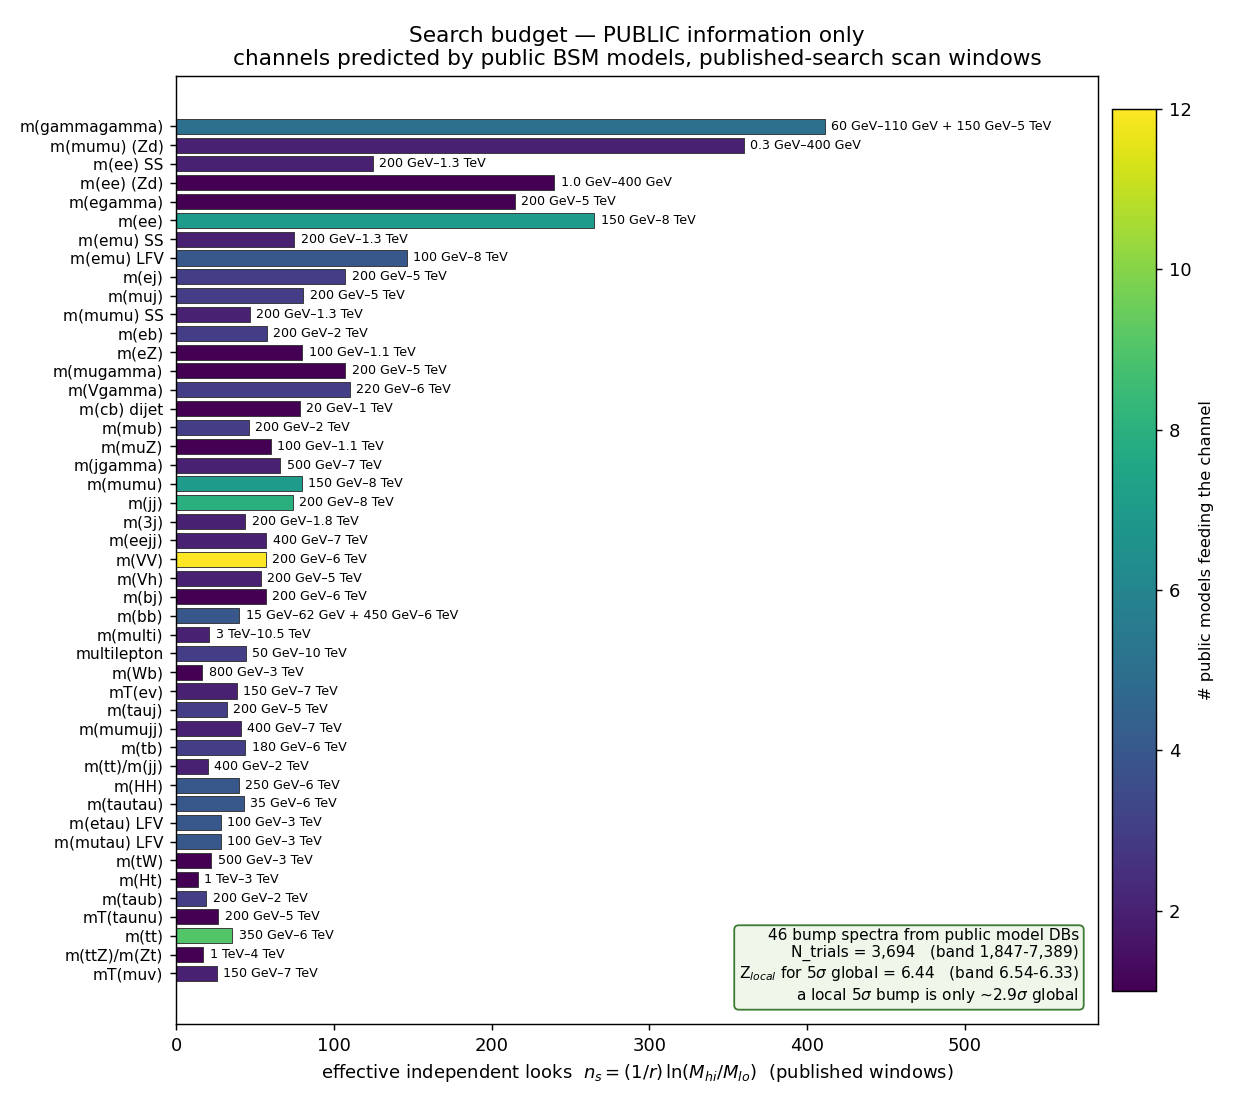
\includegraphics[width=0.92\textwidth]{search_budget.png}
\caption{Trials per spectrum, with the scan window annotated and the colour giving the number of
public model classes that feed the channel. Note the strong hierarchy: the five highest-resolution
spectra ($m(\gamma\gamma)$, the two dark-photon axes, $m(ee)$ and $m(e\gamma)$) carry $40\,\%$ of
the entire budget, simply because $n_s \propto 1/r$.}
\label{fig:budget}
\end{figure}

\subsection{Which models feed which spectrum}

The mapping from model classes to spectra is the other half of the input, and it is worth being able
to see it rather than trust it. Figure~\ref{fig:matrix} draws it in full. Two structural features
matter for the budget. First, the matrix is far from diagonal: popular spectra such as $m(jj)$,
$m(VV)$ and $\mtt$ are motivated by eight to twelve model classes each, which is exactly why the
number of \emph{searches} is so much smaller than the number of \emph{models}. Second, adding a
model to a spectrum that is already scanned costs \emph{nothing} in trials. The entire cost of
breadth sits in opening new columns, never in filling in existing ones.

\begin{figure}[htbp]
\centering
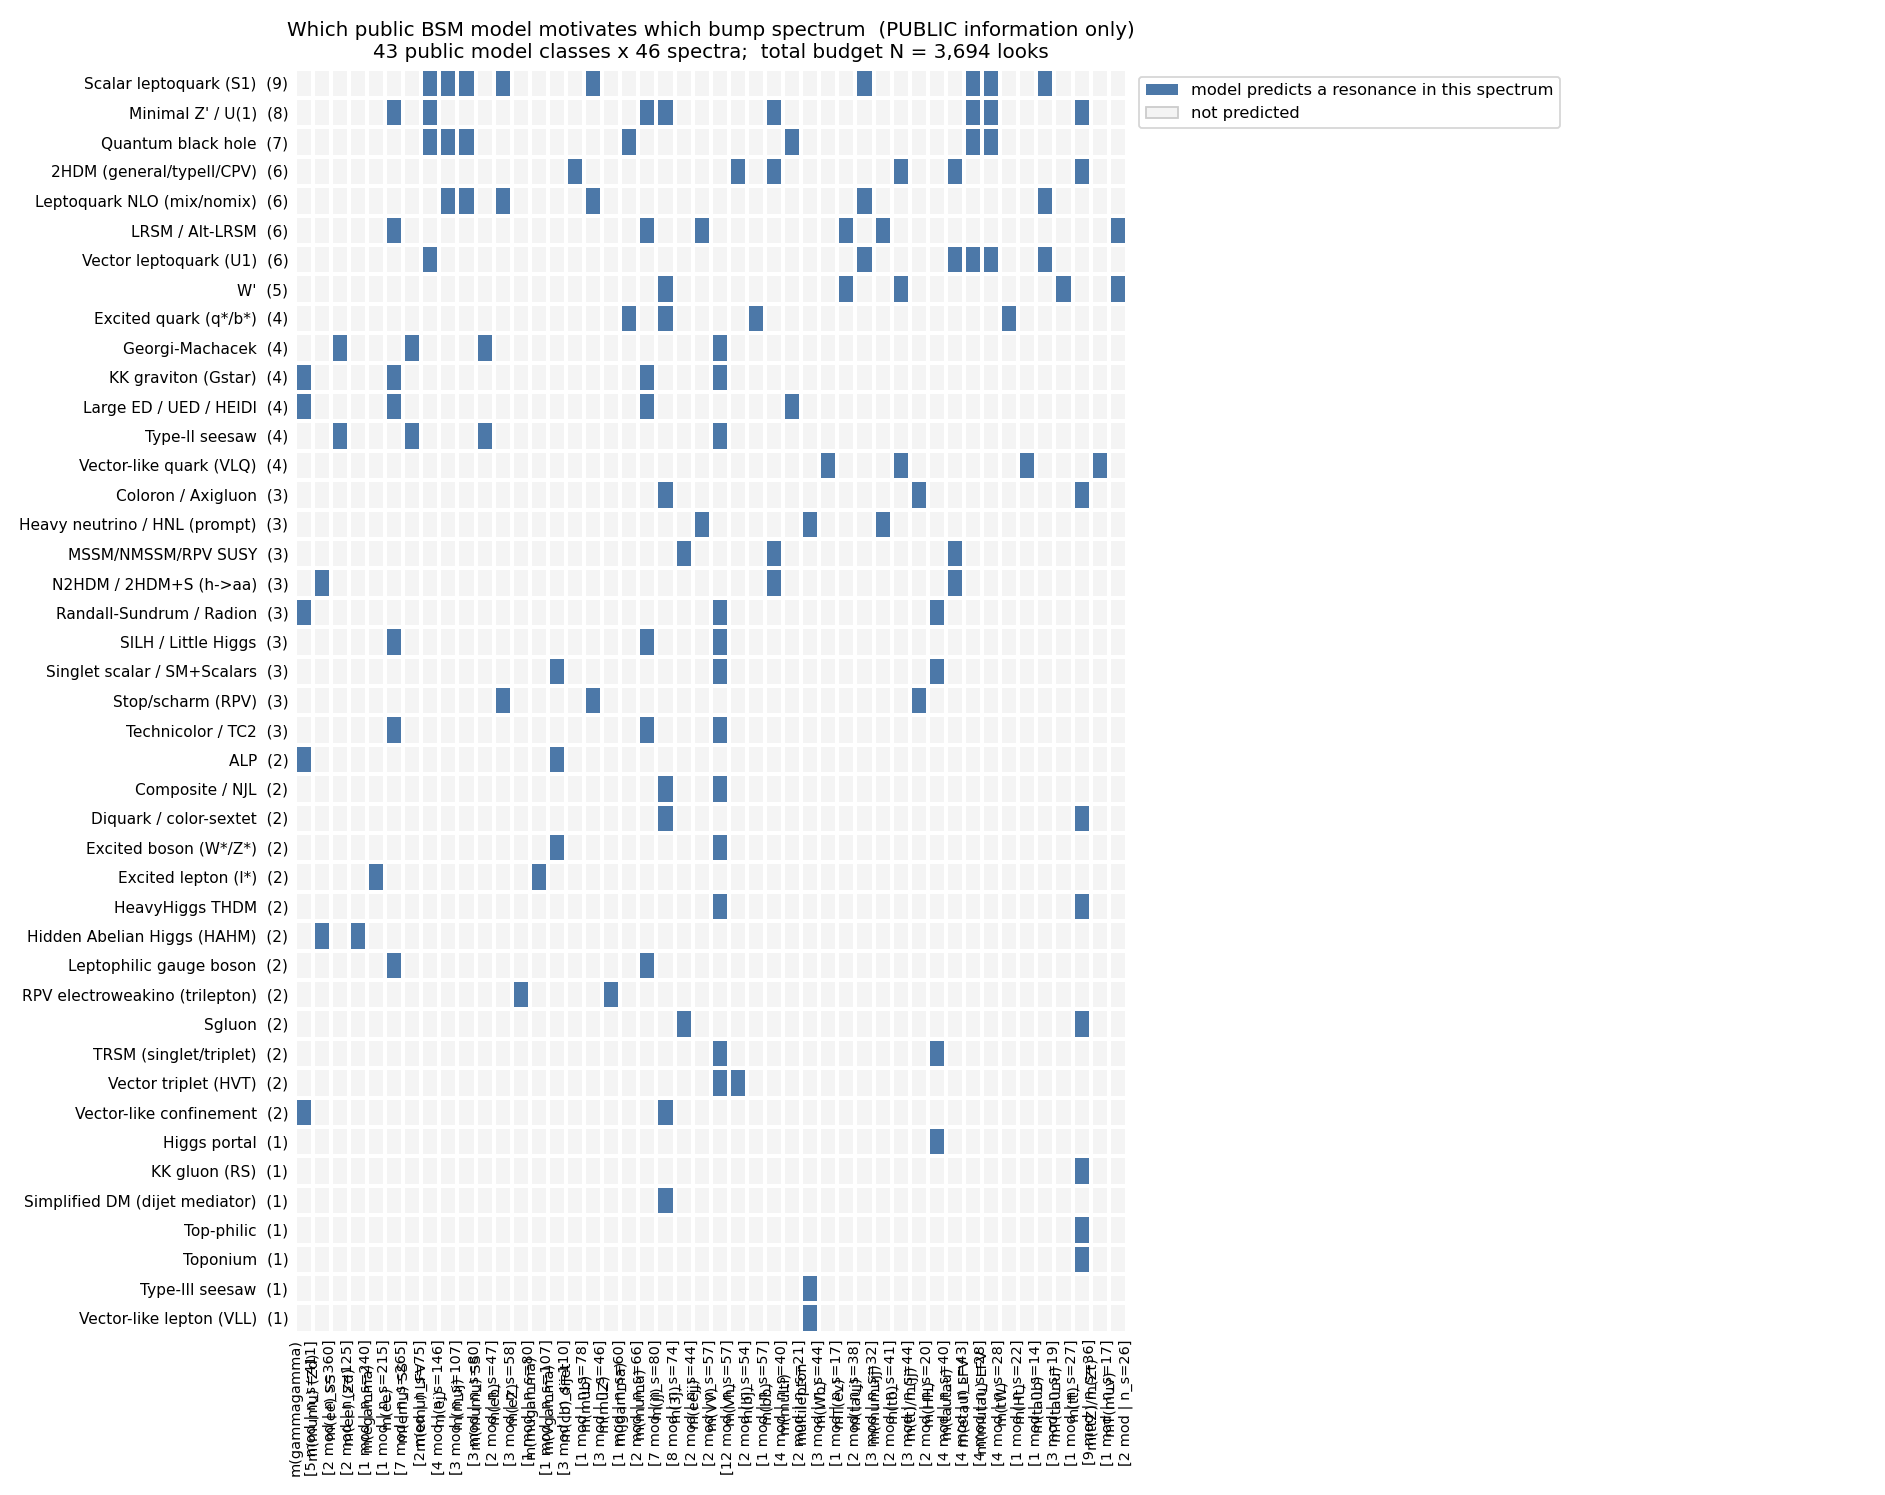
\includegraphics[width=0.95\textwidth]{model_observable_matrix.png}
\caption{Public model classes (rows) against canonical bump spectra (columns). A filled cell means
the model predicts a peak in that spectrum. The matrix is derived from the model map rather than
asserted by hand.}
\label{fig:matrix}
\end{figure}

\subsection{How finely should searches be counted?}

An inclusive count of one spectrum per observable is the lower bound. Real searches slice each
final state further, and each slice scanned for a bump is another look. Published searches split by
$b$-tag category, boosted versus resolved regime, sub-decay mode, $0/1/2$-lepton bin and ambiguous
pairing --- a leptoquark pair search scans all four lepton--jet pairings. Attaching a documented,
publication-anchored selection multiplicity to each observable gives 94 channels and
$\Nsig = 6\,616$, hence $\Zloc = 6.53$. Lepton flavour is deliberately \emph{not} one of the
multipliers, since it is already a mass axis.

\begin{table}[htbp]
\centering
\caption{The budget at increasing granularity.}
\label{tab:granularity}
\begin{tabular}{lrrr}
\toprule
granularity & spectra & $\Nsig$ & $\Zloc$ \\
\midrule
inclusive (one spectrum per observable) & 46 & 3694 & 6.44 \\
real event selections & 94 & 6616 & \textbf{6.53} \\
full ATLAS BSM program (literature, Section~\ref{sec:excess}) & --- & $\sim5\times10^4$ & 6.83 \\
\bottomrule
\end{tabular}
\end{table}

\begin{figure}[htbp]
\centering
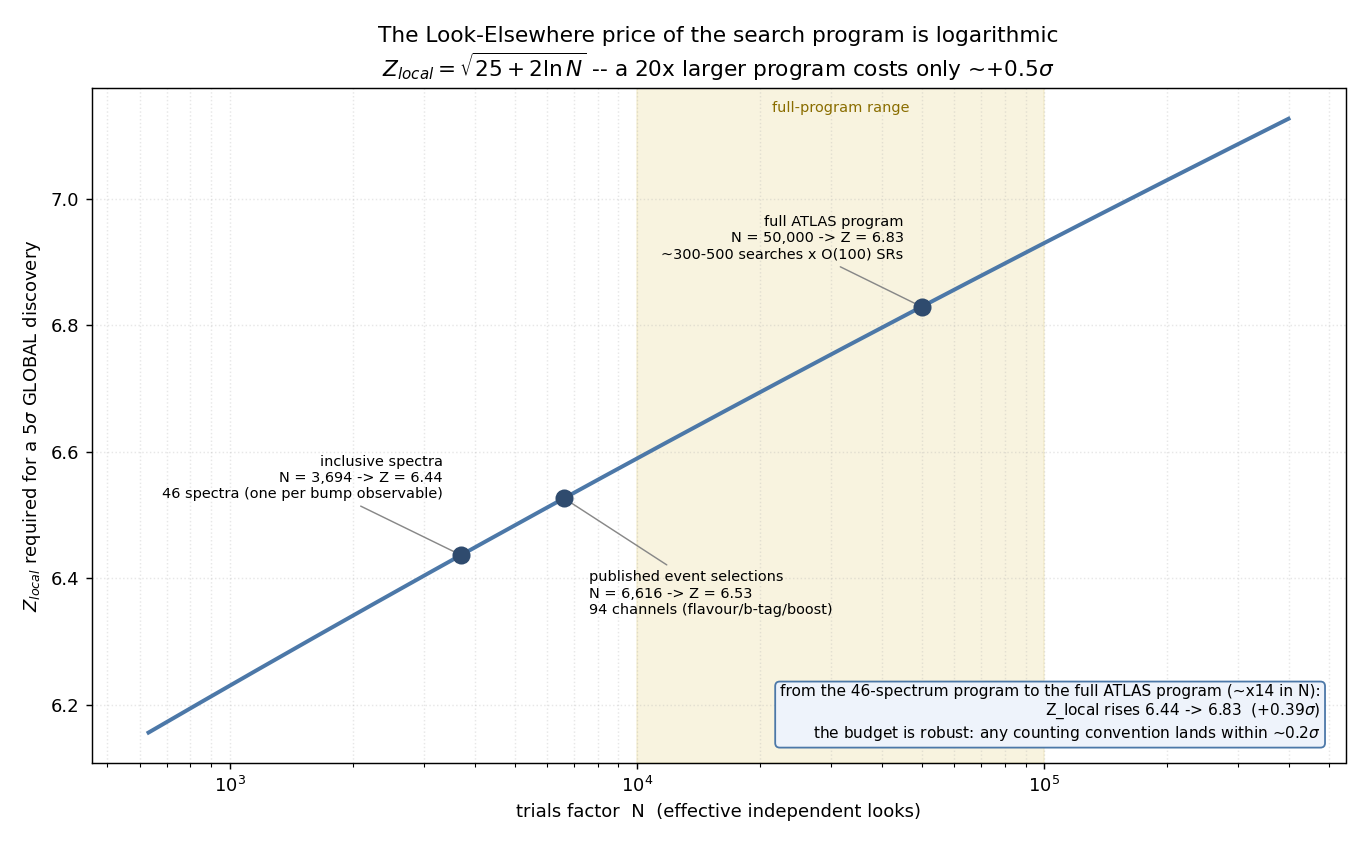
\includegraphics[width=0.88\textwidth]{budget_waterfall.png}
\caption{$\Zloc$ required for a $5\sigma$ global discovery as a function of the trials factor, with
the granularity levels of this study placed on the curve. A factor $1.8$ in channel counting moves
the discovery bar by $0.09\sigma$, and reaching the full ATLAS program, a further factor $\sim8$,
adds only another $0.3\sigma$.}
\label{fig:waterfall}
\end{figure}

\subsection{Reading the result}

The headline is robust by construction. $\Nsig$ enters only through $\ln \Nsig$, so a factor two
error in the resolution assumption, or a factor $1.8$ in how finely channels are counted, moves
the discovery bar by at most $\pm 0.1\sigma$. Every granularity level of this study in
Table~\ref{tab:granularity} sits within $0.05\sigma$ of $6.5$.

Two conclusions follow, and they pull in opposite directions.

\textbf{Breadth is cheap.} Covering the entire known BSM resonance space costs about one extra
unit of $\sigma$ relative to a single pre-specified counting experiment, $6.5$ against $5$. There
is no statistical argument for keeping the search program narrow. The marginal cost of scanning
one more spectrum is small, and the cost of adding models to an existing one is exactly zero.

\textbf{Uncountability is expensive.} The argument above works only because $\Nsig$ can be
counted. The moment the number of effective looks becomes a matter of opinion, which is the
natural state of a neural-network-driven scan, the correction one has to defend is no longer $2\ln
\Nsig$ with $\Nsig$ known but whatever a reviewer will accept. Section~\ref{sec:ab} quantifies how
much that is worth paying to avoid.

\section{The combinatorial scan, and what has never been looked at}
\label{sec:combinatorial}

Section~\ref{sec:budget} priced the program that exists: the spectra published searches scan. A
scan does not have to be restricted to those. If an analysis builds every invariant mass it can
from the objects in an event, the relevant budget is a different and much larger one, and the
difference between the two is precisely the space nobody has examined.

\subsection{Budget of a fully combinatorial scan}

To keep this concrete rather than hypothetical we fix one object budget and price it. It is the
shape a data-directed scan~\cite{ddp} of this kind naturally takes, and it is a design choice of
this note rather than a description of any particular implementation:

\begin{itemize}[leftmargin=1.4em,itemsep=2pt]
  \item Categories are \textbf{exclusive} multiplicity bins in
        $(n_e, n_\mu, n_j, n_b, n_Z, \mathrm{MET})$, so different categories select disjoint event
        sets and are statistically independent looks.
  \item The object budget is $n_e \le 2$, $n_\mu \le 2$, $n_j \le 3$, $n_b \le 3$, $n_Z \le 1$,
        with $2 \le \sum n \le 4$, missing energy excluded from the masses.
  \item A single-lepton trigger requires each populated category to contain a lepton, either a
        loose $e/\mu$ or a leptonic $Z$.
  \item Missing energy splits every category in two but never enters a mass, and two same-flavour
        loose leptons split into opposite- and same-sign.
  \item Every size-2 to size-4 subset of the indexed objects is its own histogram, so $j_0j_1$,
        $j_0j_2$ and $j_1j_2$ are three spectra rather than one.
\end{itemize}

This yields \textbf{150 exclusive multiplicity categories}, which become 204 once the
same-flavour dilepton categories are split into opposite- and same-sign, and \textbf{1094
(category, mass-group) combinations}, or 1502 histograms after that same charge split. They span 82
distinct flavour compositions. Assigning each spectrum a resolution from its object
composition ($\sigma/p_{\mathrm{T}} = 0.04$ for $e/\mu/Z$, $0.10$ for light jets and $0.20$ for
$b$-jets, combined as $r = \tfrac12\sqrt{\langle \sigma_i^2\rangle}$, which reproduces the
per-channel values used in Section~\ref{sec:budget}) and applying Eq.~\eqref{eq:ns} gives
\begin{equation*}
  \Nsig = 1.43\times10^{5}
  \qquad\Longrightarrow\qquad
  \Zloc = 6.98 \quad (\text{band } 6.88\text{--}7.08),
\end{equation*}
so a local $5\sigma$ in such a scan is worth only $1.1\sigma$ globally. Relative to the
published-program budget the trials factor grows by a factor 39 while the discovery bar moves by
$0.5\sigma$, which is the logarithm doing its work again. A combinatorial scan is not statistically
prohibitive. It is about half a sigma more expensive than the program ATLAS already runs.

\subsection{Which compositions has ATLAS actually scanned?}

Those same 82 compositions give a natural denominator for a coverage question that is normally
asked qualitatively. We map them onto the published bump observables of Appendix~\ref{app:windows}
generously, counting a composition as covered if \emph{any} published ATLAS search scans a mass
built from those object types. A published ``$V$'' is allowed to be a $Z$, a $jj$ pair or an
$\ell\ell$ pair, a published ``$t$'' to contain $b+$jets, and so on. Even on that permissive
reading:

\begin{table}[htbp]
\centering
\caption{Reachable ($\le4$-object) mass compositions with and without a published ATLAS bump hunt.
The mapping is deliberately generous, so the uncovered column is a lower bound on the gap.}
\label{tab:compgap}
\begin{tabular}{lrrr}
\toprule
multiplicity & compositions & with a published scan & with none \\
\midrule
$K=2$ & 14 & 14 & 0 \\
$K=3$ & 28 & 7 & 21 \\
$K=4$ & 40 & 4 & 36 \\
\midrule
total & 82 & 25 & \textbf{57} \\
\bottomrule
\end{tabular}
\end{table}

In this basis the gap is a pure multiplicity effect. Two-body space is saturated, while 75\,\% of
three-body and 90\,\% of four-body compositions have never been scanned. An independent audit built
from the publication record upward, in a different object basis
$\{$light jet, $b$-jet, lepton, photon$\}$, reproduces the shape: 90\,\% of two-body, 25\,\% of
three-body and roughly 11\,\% of four-body combinations scanned.

\subsection{Three reasons the covered fraction is overstated}

The generous mapping hides structure that sharpens the conclusion considerably.

\paragraph{Tag versus scan.} Several searches that look like higher-multiplicity coverage in fact
scan a two-body mass, with the extra object used only as a trigger or flavour tag. The $b$-tagged
dijet search~\cite{atlas_btag_dijet} is explicitly a two-body scan, and the dijet$+$lepton
search~\cite{atlas_dijet_lepton} scans $m_{jj}$ only. Counting either as multi-body coverage
overstates the breadth of the record.

\paragraph{Almost all mixed-flavour coverage is three papers, all since 2022.} Of roughly 45
distinct spectra ever bump-hunted by ATLAS, only about 15 are mixed-flavour or have three or more
bodies, and essentially all of those come from~\cite{atlas_ml_anomaly, atlas_multibody,
atlas_boostedz}. One of the three is a machine-learning anomaly search; the other two are
conventional scans that were simply never run before. Before 2022 that coverage was close to zero.

\paragraph{Most covered two-body spectra are covered only inside anomaly-selected phase space.}
The broadest mixed-flavour scan in the ATLAS record~\cite{atlas_ml_anomaly} covers $m_{jb}$,
$m_{je}$, $m_{be}$, $m_{j\mu}$, $m_{b\mu}$, $m_{j\gamma}$ and $m_{b\gamma}$ from $0.3$ to $8\TeV$,
but does so inside autoencoder-selected regions rather than inclusive selections. There is no
inclusive dedicated search for $m(\ell b)$, $m(\gamma b)$, or non-leptoquark $m(\ell j)$.

\subsection{The programme that was meant to cover the rest}

The ATLAS general search~\cite{atlas_general_search} populates 704 event classes, analyses 686 of
them and defines more than $10^5$ regions. It reads like blanket coverage. It is not, for a reason
that bears directly on Section~\ref{sec:budget}: it scans exactly two event-level observables per
class, $m_{\mathrm{eff}}$ and the invariant mass of \emph{all} visible objects. Class ``$1e\,2j$''
therefore yields $m_{\mathrm{inv}}(e,j,j)$ and $m_{\mathrm{eff}}$, never $m(ej)$ or $m(jj)$. The
general search is structurally blind to sub-combination masses, which is exactly where resonances
live.

The paper states the reason outright: the observable set was restricted ``to avoid a large
increase in the number of hypothesis tests''. \textbf{ATLAS declined this coverage explicitly, on
look-elsewhere grounds.} That is a deliberate trade rather than an oversight, and it is precisely
the trade the numbers above reprice. Moving from two event-level observables to all
sub-combinations shifts the discovery bar from $6.4\sigma$ to $7.0\sigma$. That is the entire cost
of the coverage the general search gave up.

Two further points on that programme. It ran on $3.2\fbinv$, which is 2015 data and 2.3\,\% of
Run~2, and it has had no successor in the event-class format. The full-Run-2 anomaly-detection
scan~\cite{atlas_ml_anomaly} is a successor in spirit, but it covers nine two-body spectra rather
than hundreds of exclusive classes.

\subsection{Named gaps}

Concrete negatives, each checked individually against the publication record rather than inferred
from the table above:

\begin{itemize}[leftmargin=1.4em,itemsep=2pt]
  \item \textbf{$m(\ell\gamma)$}, the only uncovered two-body composition in the basis. Excited
        leptons $\ell^\ast \to \ell\gamma$ were searched for at $7\TeV$~\cite{atlas_lstar_7tev} and
        $8\TeV$~\cite{atlas_lstar_8tev}; every $13\TeV$ excited-lepton search uses other channels.
  \item \textbf{Same-sign dilepton plus jets mass spectra.} $H^{\pm\pm} \to \ell^\pm\ell^\pm$ was a
        genuine same-sign mass scan at $7\TeV$~\cite{atlas_dch_7tev}, but the full-Run-2
        update~\cite{atlas_dch_run2} replaced the scan with a counting signal region.
  \item \textbf{$m(jj\gamma)$, $m(bbj)$, $m(\ell\ell j)$}, clean three-body negatives.
  \item \textbf{$m(jjjj)$}: no light-jet four-body scan. The $b$-tagged analogue \emph{is} covered,
        by the resolved $X\to HH \to 4b$ channel~\cite{atlas_hh4b}.
  \item \textbf{Colour-sextet and $E_6$ diquarks}, \textbf{$b^\ast \to b\gamma$} (CMS sets excited-bottom-quark limits in its $\gamma+$jet resonance
search~\cite{cms_gammajet}; the ATLAS $\gamma+$jet searches are flavour-inclusive), \textbf{$\tau^\ast \to \tau\gamma$} (the $\tau^\ast$ \emph{model} was
        searched through contact interactions~\cite{atlas_taustar}, so the $\tau\gamma$
        \emph{channel} is the gap), \textbf{$m(t\gamma)$}, and \textbf{same-sign $t\bar t$ as a mass
        bump}~\cite{atlas_ss_tt}: model or channel gaps with no ATLAS scan in any run.
  \item \textbf{The entire mixed-flavour $K=3$ and $K=4$ block}: $m_{jb\mu}$, $m_{ejj}$,
        $m_{e\mu b}$, $m_{eejb}$, $m_{\mu\mu bb}$ and the rest.
\end{itemize}

A fourth category turned up that is arguably more interesting than any of these, and is not
``never examined'': signatures examined once at Run-1 luminosity and then quietly abandoned.
$m(\ell Z)$~\cite{atlas_vll_8tev} and $m(Zb)$~\cite{atlas_vlq_zb_8tev} were both scanned at
$8\TeV$ and never repeated. Re-running an abandoned $8\TeV$ scan on the full Run-2 dataset costs
nothing in trials that Section~\ref{sec:budget} has not already counted.

A closing caution on how to read all of this. ``Never scanned'' is a statement about the
publication record, not about whether the signal models exist or whether samples were ever
generated for them. Those are orthogonal axes: a channel can be well supplied with theory and
simulation and still have no published scan, which is precisely the situation the table above
counts.

\section{Does the arithmetic reproduce the excesses we have seen?}
\label{sec:excess}

A trials-factor calculation is easy to get wrong in a way that is invisible. Nothing in
Section~\ref{sec:budget} would look different if $\Nsig$ were off by an order of magnitude. There
is one external check available, though, and it is a strong one. If the number of independent
looks across the ATLAS search program is known even approximately, background-only statistics
predicts how many $3\sigma$ and $5\sigma$ local excesses should have appeared. That prediction can
be compared to the historical record.

\subsection{The prediction}

The relevant count is quasi-independent statistical tests, meaning mass-resolution elements plus
signal-region bins, across all ATLAS searches rather than bump hunts alone.

\begin{table}[htbp]
\centering
\small
\caption{Trials-factor anchors for the full ATLAS search program.}
\label{tab:excess_N}
\begin{tabular}{@{}l r >{\raggedright\arraybackslash}p{6.0cm}@{}}
\toprule
level & looks $N$ & basis \\
\midrule
bump-hunt budget (public channels) & $\sim3.7\times10^3$ & this study, Section~\ref{sec:budget} \\
two-body invariant-mass searches & $\sim2$--$3\times10^4$ & $>50\,000$ LHC-wide~\cite{statinterp}, ATLAS $\sim$ half \\
full ATLAS BSM program (incl.\ SRs) & $\sim5\times10^4$ & $300$--$500$ searches $\times\,\mathcal{O}(100)$ regions~\cite{diggingdeeper} \\
\bottomrule
\end{tabular}
\end{table}

With a one-sided Gaussian tail, $p(\ge3\sigma) = 1.35\times10^{-3}$ and $p(\ge5\sigma) =
2.87\times10^{-7}$, the expected counts are $N \cdot p$:

\begin{table}[htbp]
\centering
\caption{Expected upward fluctuations under background-only.}
\label{tab:excess_expected}
\begin{tabular}{lrr}
\toprule
$N$ & expected $\ge3\sigma$ & expected $\ge5\sigma$ (spurious) \\
\midrule
$10^4$ & 14 & 0.003 \\
$5\times10^4$ (central) & \textbf{67} & \textbf{0.014} \\
$10^5$ & 135 & 0.029 \\
resonance subset, $3.7\times10^3$ & 5.0 & $1.1\times10^{-3}$ \\
\bottomrule
\end{tabular}
\end{table}

\begin{figure}[htbp]
\centering
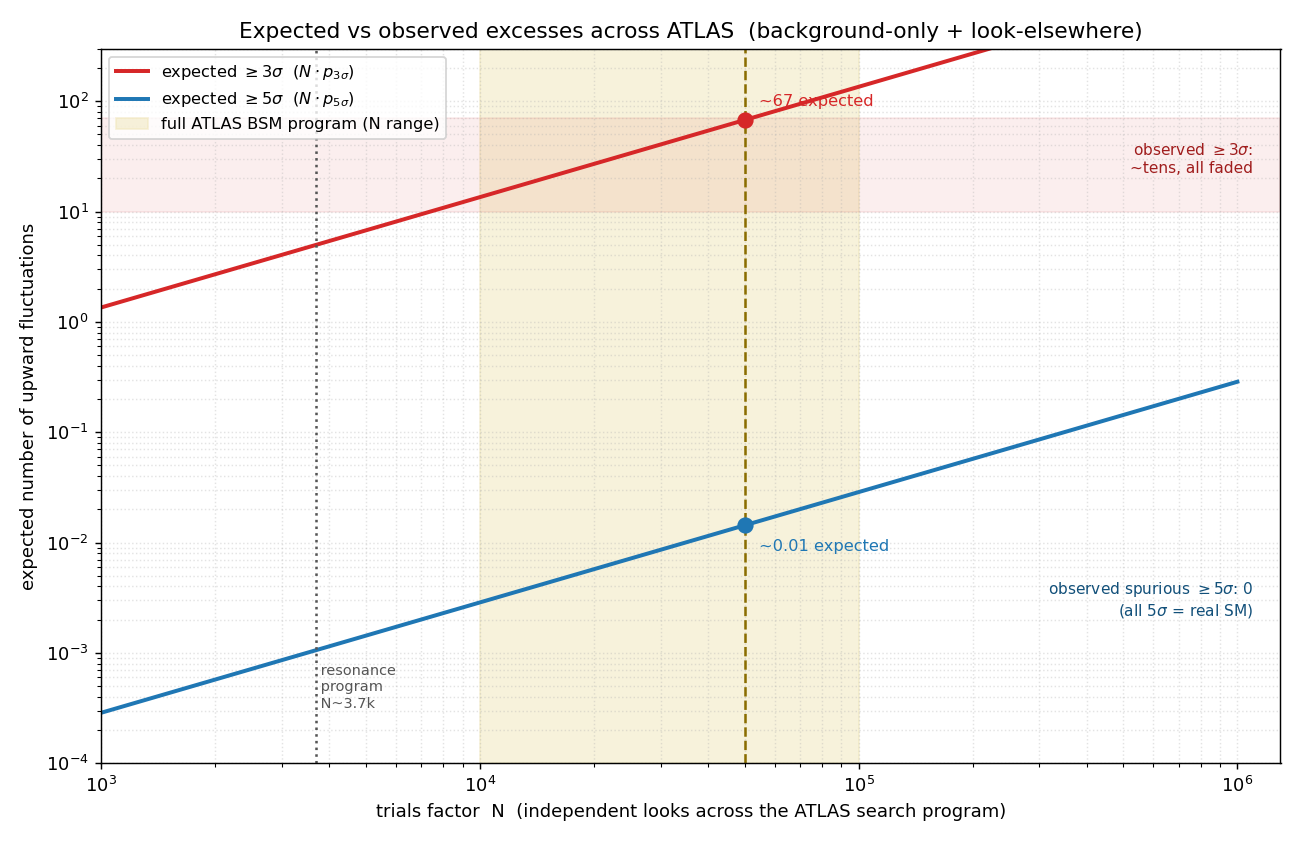
\includegraphics[width=0.85\textwidth]{excess_counting.png}
\caption{Expected number of upward fluctuations above $Z$ as a function of the number of
independent looks, with the anchors of Table~\ref{tab:excess_N} marked. The $\ge5\sigma$ curve
stays below unity across the entire defensible range of $N$, which is the quantitative content of
the $5\sigma$ convention~\cite{lyons2008}.}
\label{fig:excess}
\end{figure}

\subsection{The record}

\textbf{At $3\sigma$: order tens, essentially all faded.} The $750\GeV$ diphoton excess
($3.9\sigma$ local in 2015, $2.1\sigma$ global, gone with more data), the $2\TeV$ diboson $WZ$
excess at $8\TeV$, the $95\GeV$ and $151\GeV$ diphoton hints, the multilepton anomalies, a
$400\GeV$ $t\bar t$ excess, and the surviving $\sim3\sigma$ excesses found hiding inside published
SUSY signal regions~\cite{diggingdeeper}. That is the expected population, not a mystery.

\textbf{At $5\sigma$: every one is a genuine Standard-Model process.} The Higgs boson, four-top
production, $t\bar tZ$/$t\bar tW$/$t\bar tH$, vector-boson scattering, single top; the public
summary of ATLAS search results~\cite{atlas_public_searches} contains no BSM counterexample.
\textbf{Spurious BSM $\ge5\sigma$: exactly zero.} Four-top production is instructive rather than a
counterexample: it evolved from $3\sigma$ to $5\sigma$ and turned out to be real.

\subsection{Verdict}

\begin{table}[htbp]
\centering
\caption{Expected versus observed, for $N \sim 5\times10^4$.}
\label{tab:excess_verdict}
\begin{tabular}{lrl}
\toprule
 & expected & observed \\
\midrule
$\ge3\sigma$ local & $\sim15$--$135$ & order tens, all faded \\
$\ge5\sigma$ spurious & $\sim0.01$ & 0 \\
\bottomrule
\end{tabular}
\end{table}

The two agree. This matters for the note's central claim in a specific way: the same
look-elsewhere arithmetic that produces $\Zloc \approx 6.4$ in Section~\ref{sec:budget} also
post-dicts the observed excess population without adjustment. The framework is at least
self-consistent, and the parade of $3\sigma$ hints that come and go needs no explanation beyond $N
\times p$.

The corollary is uncomfortable. With more than $50\,000$ looks LHC-wide, a local $5\sigma$ in a
fully agnostic scan is worth only $1.5$ to $2.5\sigma$ globally, which is the basis of the
argument~\cite{statinterp} for raising the agnostic-scan threshold towards $7\sigma$. This note
reaches essentially the same number from the opposite direction for a combinatorial scan
(Section~\ref{sec:combinatorial}, $\Zloc = 6.98$).

Three caveats. $N$ spans a factor ten and is the dominant uncertainty here, although the
conclusion survives the whole range. The counts mix ATLAS-only and ATLAS$+$CMS excesses. And
``order tens observed'' counts \emph{notable} excesses; the raw number of individual $\ge3\sigma$
bins is much larger and goes unremarked, which is also consistent, since those are the expected
noise.

\section{Selecting candidates from a scan}
\label{sec:selection}

Sections~\ref{sec:budget} and~\ref{sec:combinatorial} priced the scan. This section asks what to
do with its output. A broad scan produces a large number of local significances, one per bin per
spectrum, and something has to decide which of them is worth following up. Three rules are
compared here on identical footing: take the largest (\emph{argmax}), take everything above a
fixed threshold, or let the data set the cut through a false-discovery-rate criterion.

The setting is deliberately minimal: $n = 30\,000$ bins, of which $n-1$ are background with $z_i
\sim \mathcal{N}(0,1)$, and at most one contains a signal with $z \sim \mathcal{N}(\mu, 1)$.
Whatever passes stage 1 is unblinded in an independent sample B and confirmed if $z_B > 3$. This
is the two-stage structure of Section~\ref{sec:ab} stripped to its statistical core.

\subsection{The background maximum is not Gaussian}

The first thing to get right is the null distribution of $\max_i z_i$. Two limits are routinely
confused. Running more pseudo-experiments makes the histogram converge to the \emph{exact} density
\begin{equation}
  f_M(x) \;=\; n\,\phi(x)\,\Phi(x)^{n-1},
  \qquad
  F_M(x) = \Phi(x)^n,
  \qquad
  x_q = \Phi^{-1}\!\left(q^{1/n}\right),
  \label{eq:maxexact}
\end{equation}
which is exact for every $n$. Increasing $n$ makes the \emph{rescaled} $f_M$ converge to a Gumbel
law~\cite{fishertippett,gumbel}, and that convergence is only logarithmic, with relative error
$\mathcal{O}(1/2\ln n)$.

At $n = 30\,000$ the difference is measurable, and $10^4$ pseudo-experiments are enough to resolve
it (Table~\ref{tab:maxvalidation}). The exact form is confirmed; the asymptotic Gumbel is rejected
at $p = 2\times10^{-15}$ and a best-fit Gaussian at $p = 6\times10^{-30}$.

\begin{table}[htbp]
\centering
\caption{Distribution of the maximum of $n=30\,000$ standard normals, from $10^4$
pseudo-experiments, against the exact law and its Gumbel limit
($a_n = 4.005$, $b_n = 0.220$).}
\label{tab:maxvalidation}
\begin{tabular}{lrr}
\toprule
 & simulated & Gumbel asymptotic \\
\midrule
mean & 4.110 & 4.132 \\
standard deviation & 0.284 & 0.282 \\
median & 4.072 & 4.086 \\
skewness & 0.89 & 1.14 \\
\midrule
KS vs exact $\Phi(x)^n$ & \multicolumn{2}{r}{$D = 0.0077$, $p = 0.59$ \quad\checkmark} \\
KS vs Gumbel$(a_n,b_n)$ & \multicolumn{2}{r}{$D = 0.041$, $p = 2\times10^{-15}$} \\
KS vs best-fit Gaussian & \multicolumn{2}{r}{$D = 0.058$, $p = 6\times10^{-30}$} \\
\bottomrule
\end{tabular}
\end{table}

\begin{figure}[htbp]
\centering
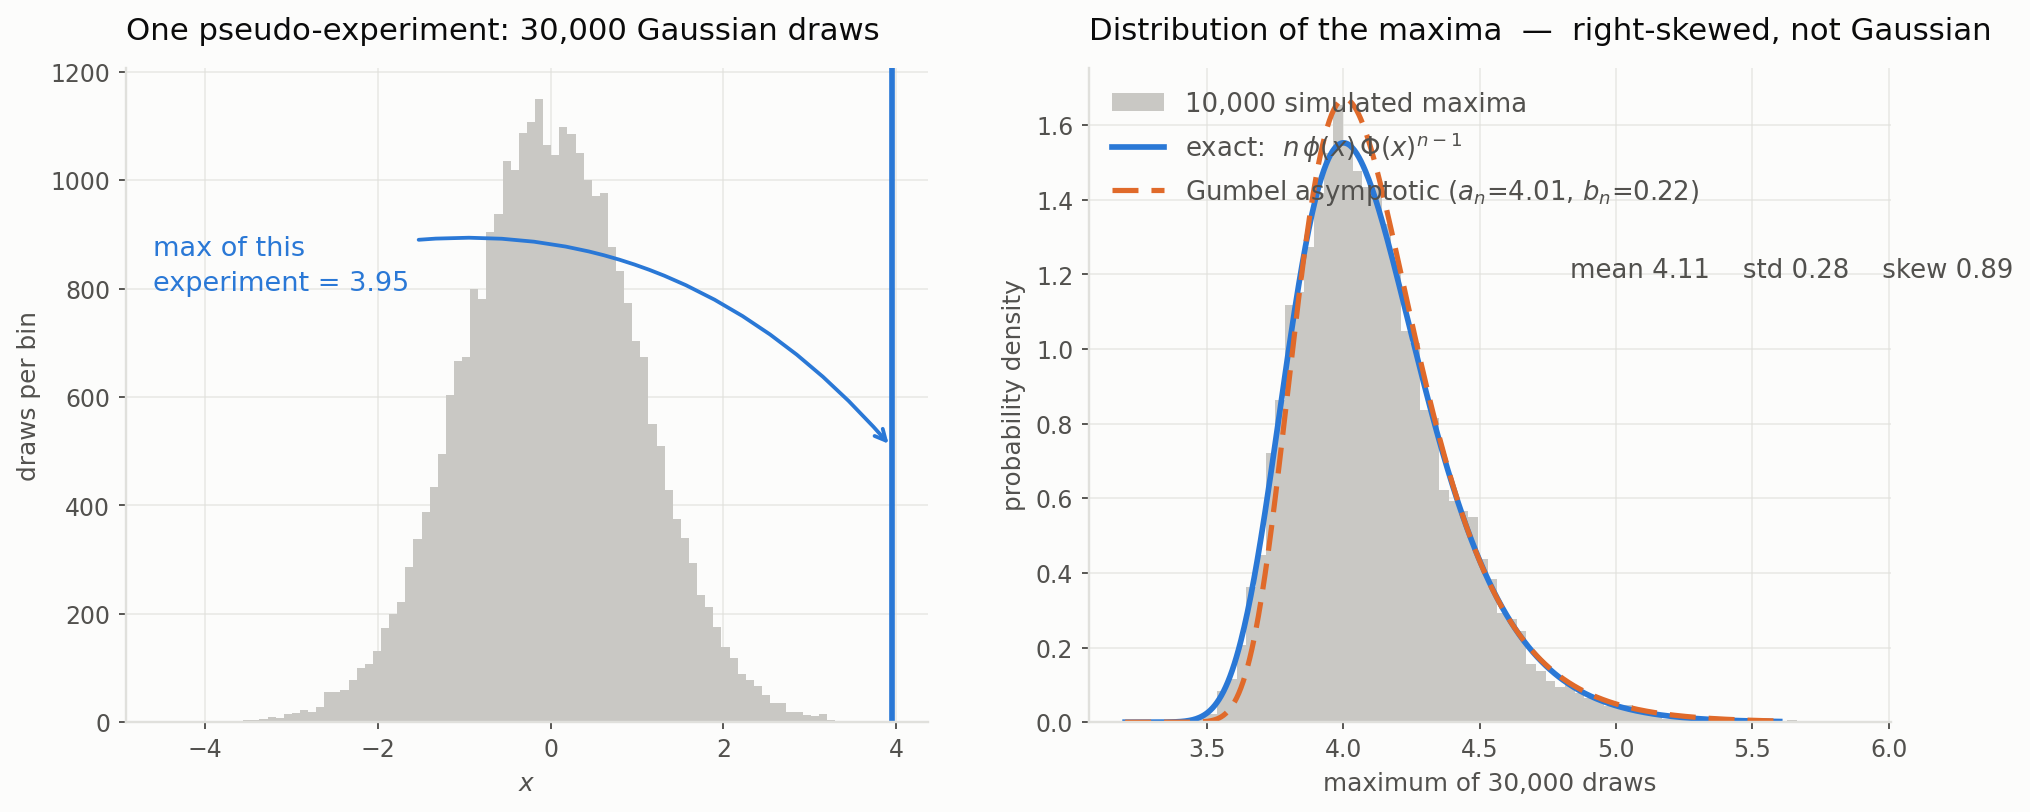
\includegraphics[width=0.95\textwidth]{max_of_gaussians_light.png}
\caption{Left: one pseudo-experiment of $30\,000$ Gaussian draws, with its maximum marked. Right: the
distribution of $10^4$ such maxima, with the exact density of Eq.~\eqref{eq:maxexact} and the
asymptotic Gumbel overlaid. The distribution is strongly right-skewed, so a symmetric error bar on
a maximum is never appropriate.}
\label{fig:maxgauss}
\end{figure}

The practical rules that follow are short. Gumbel is fine for intuition. For any actual number,
whether a threshold, a $p$-value or a quantile, use $F_M = \Phi^n$, which costs nothing and is
right. Never model a maximum as Gaussian. This also connects back to Section~\ref{sec:budget}: the
familiar trials factor is the leading term of $1 - \Phi(z)^{N_{\mathrm{eff}}}$, and in the far
tail, where global $p$-values live, a few-percent Gumbel error is not something one wants between
oneself and a discovery claim.

\subsection{A real signal often loses the scan}

The probability that the signal bin \emph{is} the maximum, $p(\mu) = \int
\phi(s-\mu)\,\Phi(s)^{n-1}\,\mathrm{d}s$, is sobering. A genuine $4\sigma$ signal wins the scan
only 46\,\% of the time, because it is racing a distribution centred at $4.11$ with a spread of
$0.28$. The two-stage confirmation probability follows as
$p_{\mathrm{conf}} = p(\mu)\,\Phi(\mu - 3) + [1-p(\mu)]\,\Phi(-3)$ (Table~\ref{tab:rules}).

The second stage is nearly free. For $\mu \ge 5\sigma$ the loss between ``wins the scan'' and
``confirmed'' is under two percentage points, because a signal strong enough to win stage 1 almost
always exceeds $3\sigma$ in stage 2. \textbf{Stage 2 also carries no trials factor}, since the bin
was chosen by stage 1. The false-alarm rate per opening is $1-\Phi(3) = 1.35\times10^{-3}$, or
$3.0\sigma$ \emph{global}, whatever the size of the scan that selected it.

\subsection{A threshold dominates the argmax}

Taking the maximum throws information away: it ranks bins and then discards everything about their
absolute size. The alternative is to select every bin above a fixed threshold $t$. Under
background-only the number selected is Poisson with mean $\lambda(t) = (n-1)\,[1-\Phi(t)]$, so the
natural operating point is $t^\star = \Phi^{-1}(1 - 1/(n-1)) = 3.99$, where $\lambda = 1$. That is
exactly the argmax's fake budget of one candidate per experiment, and at that matched budget the
threshold rule wins at every signal strength (Table~\ref{tab:rules}).

\begin{table}[htbp]
\centering
\caption{Probability that a signal of strength $\mu$ is confirmed in sample B, for the three
stage-1 rules, all at the same background-only budget of one candidate per experiment
($3.0\sigma$ global false-alarm rate). The threshold operating point is $t^\star = 3.99$ and the
matched false-discovery rate is $q^\star = 0.381$.}
\label{tab:rules}
\begin{tabular}{lrrrr}
\toprule
$\mu$ & wins the scan & argmax confirmed & BH at $q^\star$ & threshold at $t^\star$ \\
\midrule
$3\sigma$ & 14.2\,\% & 7.2\,\% & 7.5\,\% & \textbf{8.1\,\%} \\
$4\sigma$ & 45.8\,\% & 38.6\,\% & 40.3\,\% & \textbf{42.5\,\%} \\
$5\sigma$ & 80.3\,\% & 78.5\,\% & 80.6\,\% & \textbf{82.5\,\%} \\
$6\sigma$ & 96.4\,\% & 96.3\,\% & 97.2\,\% & \textbf{97.7\,\%} \\
\bottomrule
\end{tabular}
\end{table}

Putting both rules on a common ROC, with the average number of false confirmations on one axis and
the signal confirmation probability on the other, makes the structure clear
(Figure~\ref{fig:roc}). The threshold rule traces a curve as $t$ varies. The argmax is a
\emph{single point}, because it always selects exactly one bin, and that point lies strictly
inside the curve at every $\mu$. It is dominated, not merely different.

One caveat took some care to get right. The bare ratio of power to false positives has no interior
maximum; it increases monotonically with $t$ and simply says ``cut harder''. The well-posed
question is where the ROC tangent has a given slope, which amounts to saying what a false positive
costs relative to a discovery. Once that cost is specified, the optimum has a closed form.

\begin{figure}[htbp]
\centering
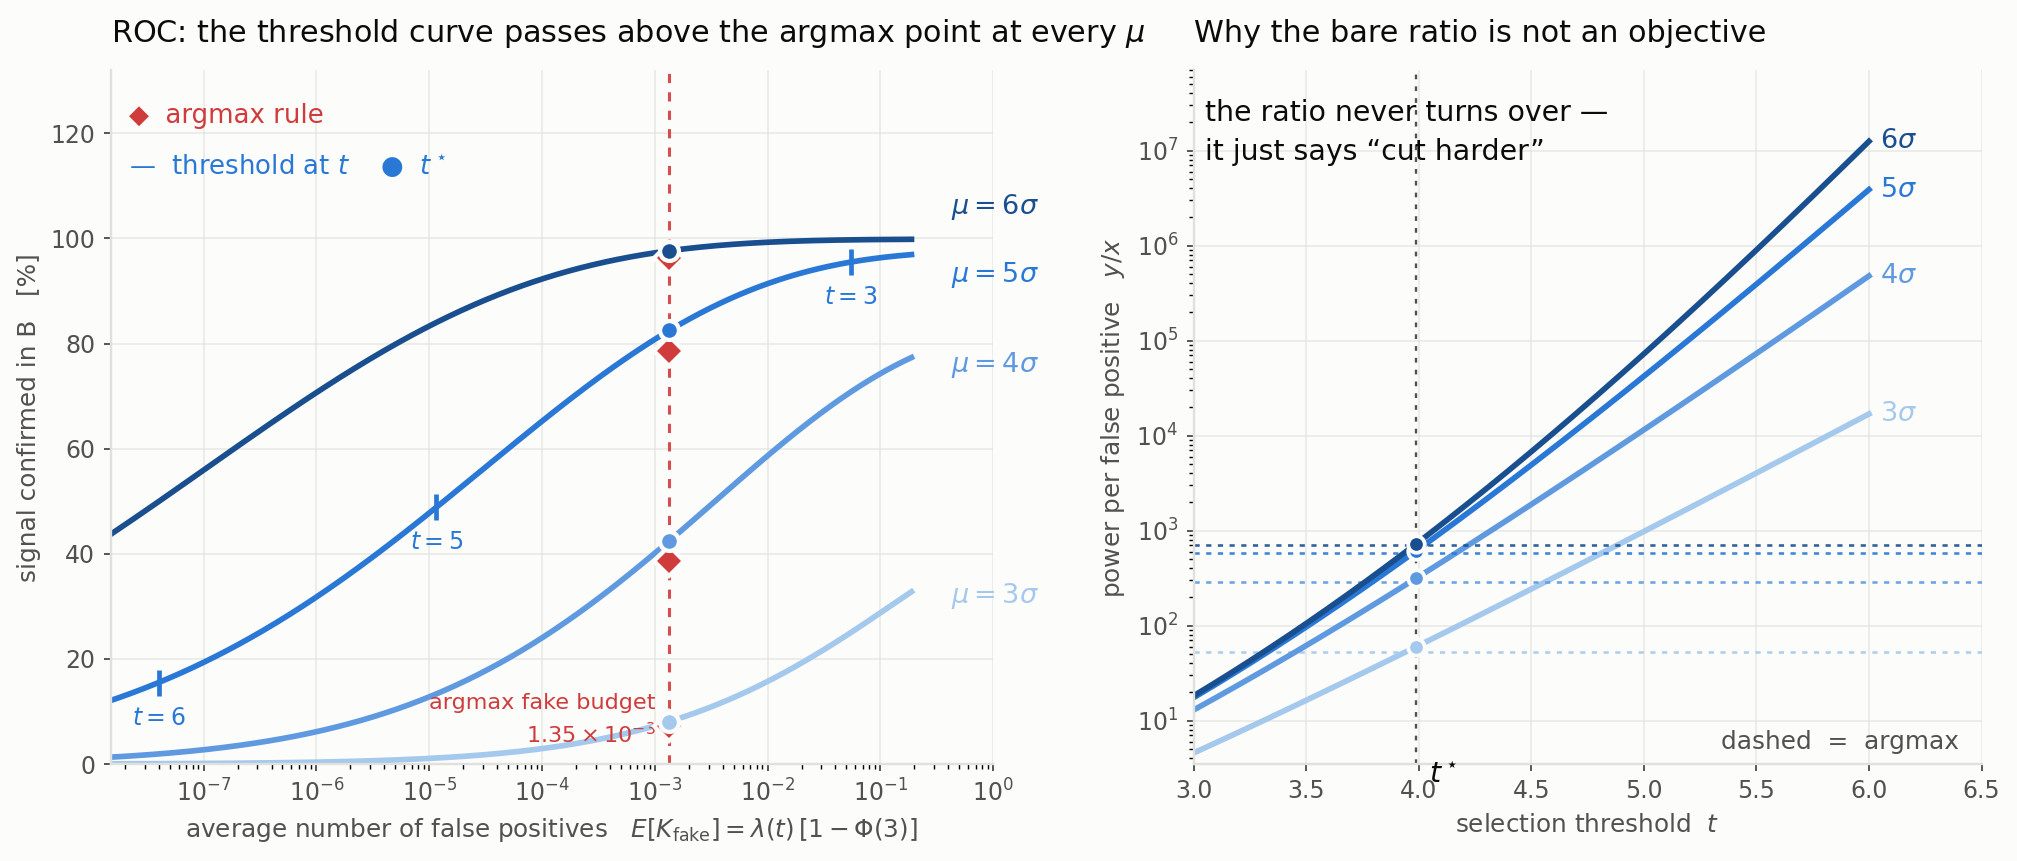
\includegraphics[width=0.95\textwidth]{roc_threshold_vs_argmax.png}
\caption{Left: the ROC of the threshold rule (one curve per signal strength) with the argmax rule as a
single point (diamonds), at $\mu = 3, 4, 5, 6\sigma$. The argmax point lies inside the curve at
every $\mu$, so at the same false-positive budget a threshold confirms more signal. Right: the
bare power-per-false-positive ratio, which never turns over. An objective has to specify what a
false positive costs.}
\label{fig:roc}
\end{figure}

\subsection{Letting the data set the cut: Benjamini--Hochberg}

The third rule replaces a fixed bar with a false-discovery-rate
criterion~\cite{benjaminihochberg}. Convert each bin to a one-sided $p$-value, sort, and reject
the $K(q)$ smallest, where $K(q) = \max\{k : p_{(k)} \le kq/n\}$. The dial is now $q$, the nominal
FDR. Since $K$ is a random variable depending on the whole $p$-vector, this has to be evaluated by
Monte Carlo.

Two properties matter here. First, under the global null the probability that BH makes at least one rejection is exactly $q$.
This follows from the identity $P(\sup_t F_n(t)/t \ge 1/q) = q$ for the uniform empirical
distribution, usually attributed to Daniels~\cite{daniels}, and our Monte Carlo reproduces it ($q
= 0.05 \to 0.0505$, $0.2 \to 0.1990$, $0.5 \to 0.5008$). The \emph{number} of rejections is not $q$: BH is
bursty, and past $q^\star$ multi-rejection events dominate. Second, the realised cut is not fixed.
In a pseudo-experiment where BH rejects $K$ bins the weakest accepted bin sits at
$z_{\mathrm{cut}} = \Phi^{-1}(1-p_{(K)})$, which fluctuates from experiment to experiment.

Matching BH to the same fake budget as the other two rules, $E[K \mid H_0] = 1$, gives $q^\star =
0.381$, and it then agrees on both false-alarm measures ($1.34\times10^{-3}$ expected false
confirmations and $P(\ge1) = 1.336\times10^{-3}$, which is $3.0\sigma$ global). Its effective
single-bin bar is $z_1(q^\star) = 4.21$, \emph{stricter} than $t^\star = 3.99$.

BH lands strictly between the other two rules (Table~\ref{tab:rules}, Figure~\ref{fig:rocbh}). It
beats the argmax for the same reason the threshold does: it never discards the signal candidate
merely because some background bin happened to be larger, and the step-up lets a signal ride along
at rank 2 or below. It loses to the fixed threshold because keeping $E[K\mid H_0] = 1$ while
spending part of that budget on rank-$2+$ clumps forces the single-bin bar up to $4.21$, and those
extra selections are pure waste. They are background bins, and the signal, normally rank 1, gains
nothing from them. The effect is specific to large $q$; at small $q$ BH is essentially the rank-1
bar and the three rules converge.

\begin{figure}[htbp]
\centering
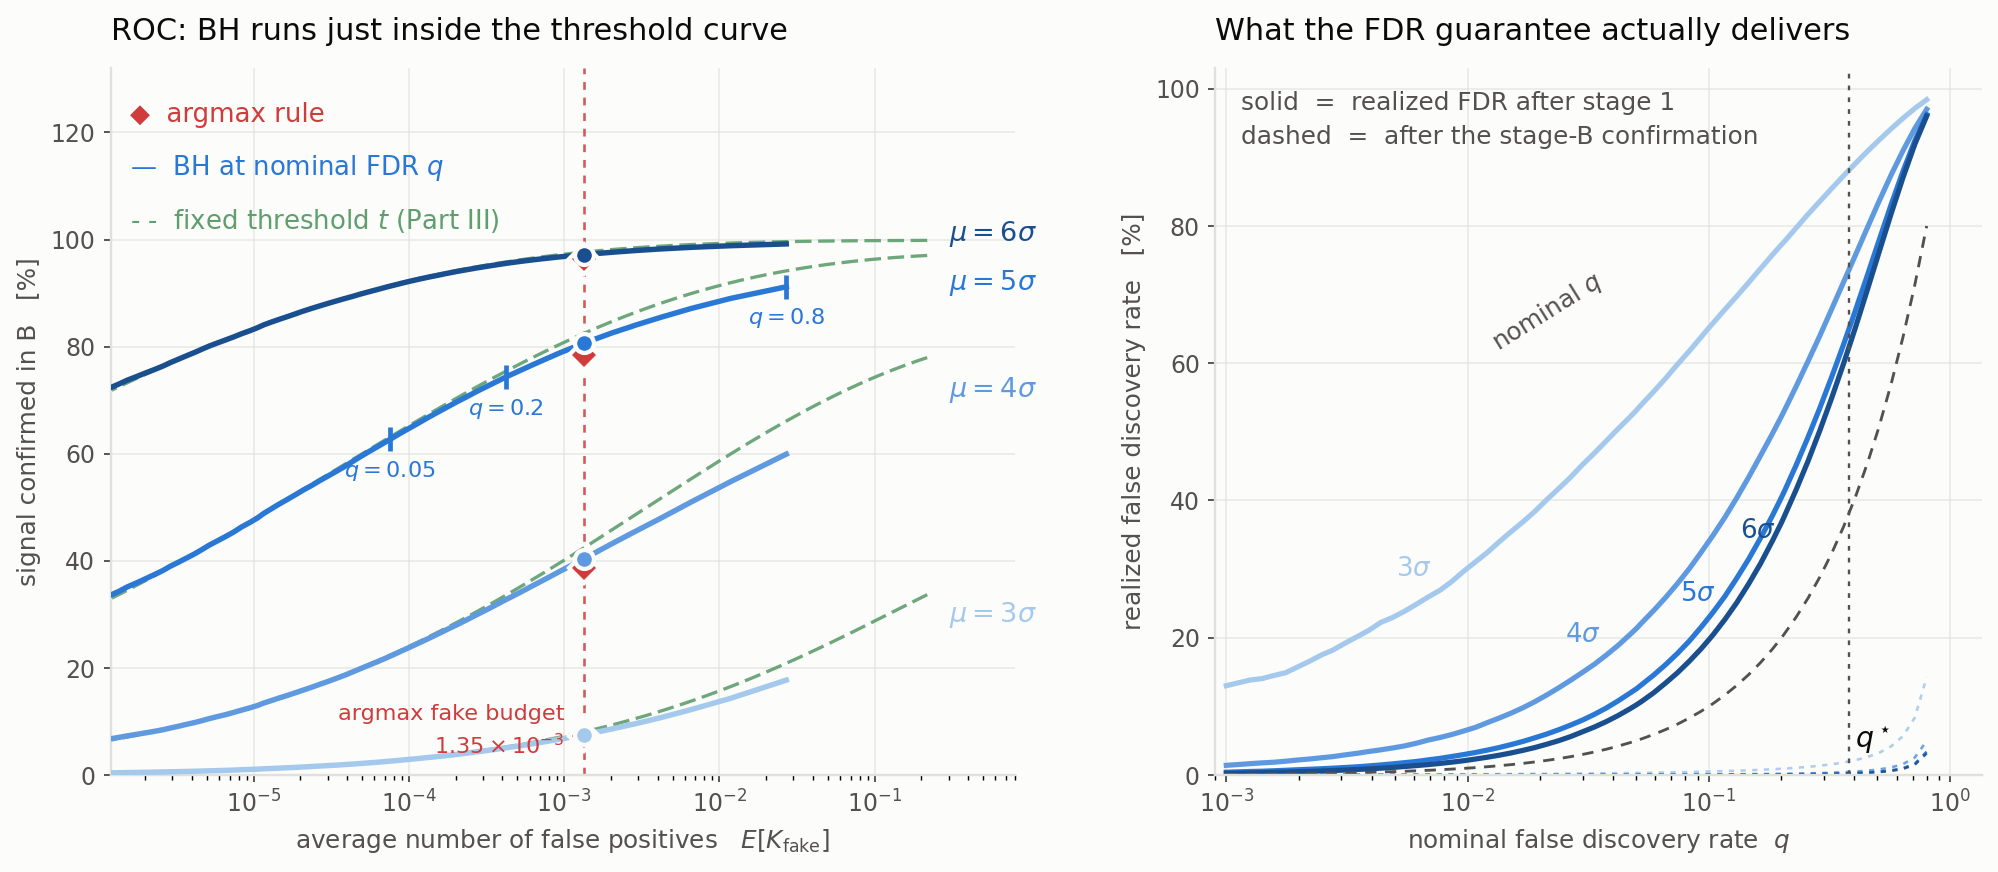
\includegraphics[width=0.95\textwidth]{roc_bh_vs_threshold.png}
\caption{Left: all three stage-1 rules on the ROC of Figure~\ref{fig:roc}. BH runs just inside the
fixed-threshold curve and outside the argmax point. Right: the realised false discovery rate
before and after the stage-B confirmation. The confirmation step drives it to near zero regardless
of the nominal $q$.}
\label{fig:rocbh}
\end{figure}

\subsection{The same three rules with an imperfect estimator}
\label{sec:selnoise}

Everything above assumes the estimator returns $z \sim \mathcal{N}(0,1)$ for every background bin.
Section~\ref{sec:abnoise} argues that a network-driven scan does not have that estimator, and the
comparison is worth redoing with the same defect model, because the three rules are not equally
exposed to it. The exposure is structural rather than numerical: argmax and BH are
\textbf{rank-based}, so an artefact anywhere in the scan changes the decision about every other
bin, while a fixed threshold is \textbf{absolute} and an artefact at 1\,TeV says nothing about the
bin at 3\,TeV.

Table~\ref{tab:selnoise} redoes Table~\ref{tab:rules} at $\mu = 5\sigma$, with every rule tuned to
the \emph{same} $3.0\sigma$-global false-alarm budget under each contamination. The
$\epsilon = 0$ row reproduces the perfect-estimator result, which fixes the comparison.

\begin{table}[htbp]
\centering
\caption{Probability that a $5\sigma$ signal is confirmed, for the three stage-1 rules, all held
at $1.35\times10^{-3}$ expected false confirmations. \textsc{glitch} and \textsc{bias} are the
incoherent and coherent defect classes of Section~\ref{sec:abnoise}. ``n/a'' means the rule cannot
be tuned to that budget at all. Monte-Carlo error on the BH column is $\pm0.35$ points; the other
two are analytic.}
\label{tab:selnoise}
\begin{tabular}{lrrrrr}
\toprule
estimator & argmax & threshold & BH & thr $-$ argmax & thr $-$ BH \\
\midrule
perfect (Table~\ref{tab:rules}) & 78.5\,\% & \textbf{82.5\,\%} & 80.9\,\% & $+4.0$ & $+1.6$ \\
\textsc{glitch} $\epsilon = 10^{-4}$ & 73.2\,\% & \textbf{81.2\,\%} & 80.1\,\% & $+8.0$ & $+1.1$ \\
\textsc{glitch} $\epsilon = 10^{-3}$ & 43.8\,\% & \textbf{57.3\,\%} & 57.2\,\% & $+13.6$ & $+0.1$ \\
\textsc{glitch} $\epsilon = 10^{-2}$ & 6.2\,\% & 5.8\,\% & 6.0\,\% & $-0.4$ & $-0.2$ \\
\textsc{bias}, any $\epsilon$ & \emph{untunable} & $\sim 0\,\%$ & \emph{unreachable} & --- & --- \\
\bottomrule
\end{tabular}
\end{table}

\paragraph{The threshold's margin over the argmax widens, from $+4$ to $+13.6$ points.} The cause
is visible in a single diagnostic: the probability that the argmax \emph{is} the signal falls from
$80.3\,\%$ to $74.9\,\%$ to $44.8\,\%$ as $\epsilon$ runs from $0$ to $10^{-3}$. At $\epsilon =
10^{-3}$ some thirty artefact bins are scattered through a $30\,000$-bin scan, and any one of them
outranking the signal removes it completely. A rank-1 rule has no graceful degradation, whereas a
threshold pays only through the extra candidates it forwards.

\paragraph{Contamination strips BH of the adaptivity that made it attractive.} BH converges onto
the fixed threshold ($+1.6 \to +1.1 \to +0.1$), and the reason is mechanical: to hold the
false-alarm budget it has to be run at ever smaller $q$, and BH at small $q$ simply \emph{is} a
threshold at $\Phi^{-1}(1-q/n)$. One keeps the threshold's performance while losing the ability to
interpret the dial.

\paragraph{And that dial becomes actively misleading.} The nominal $q$ needed to buy the same
$3.0\sigma$-global rate runs $0.38 \to 0.32 \to 1.4\times10^{-2} \to 4.2\times10^{-7}$ across the
rows of Table~\ref{tab:selnoise} (Fig.~\ref{fig:selnoise}, middle). Under coherent defects it
cannot be bought at all: even $q = 10^{-9}$ leaves $2.5\times10^{-3}$ expected false confirmations
at $\epsilon = 10^{-4}$, rising to $0.25$ at $\epsilon = 10^{-2}$, because a coherent artefact
carries a $p$-value small enough to be rejected at essentially any $q$ and then confirms in stage
2. Nothing here contradicts the FDR guarantee --- BH controls the false discovery rate under the
null it is handed, and a contaminated scan does not hand it that null.

\paragraph{The argmax should be dropped rather than deprioritised.} It has no tuning parameter, so
its false-alarm rate is whatever the contamination makes it: $1.35\times10^{-3} \to 0.137 \to
0.687 \to 0.957$ under coherent defects (Fig.~\ref{fig:selnoise}, right). At $\epsilon = 10^{-2}$
the argmax rule produces a false confirmation in $96\,\%$ of scans and there is no way to dial it
back. Under incoherent defects it stays at $1.35\times10^{-3}$, since a glitch dies in stage 2, and
only the power collapses.

\begin{figure}[htbp]
\centering
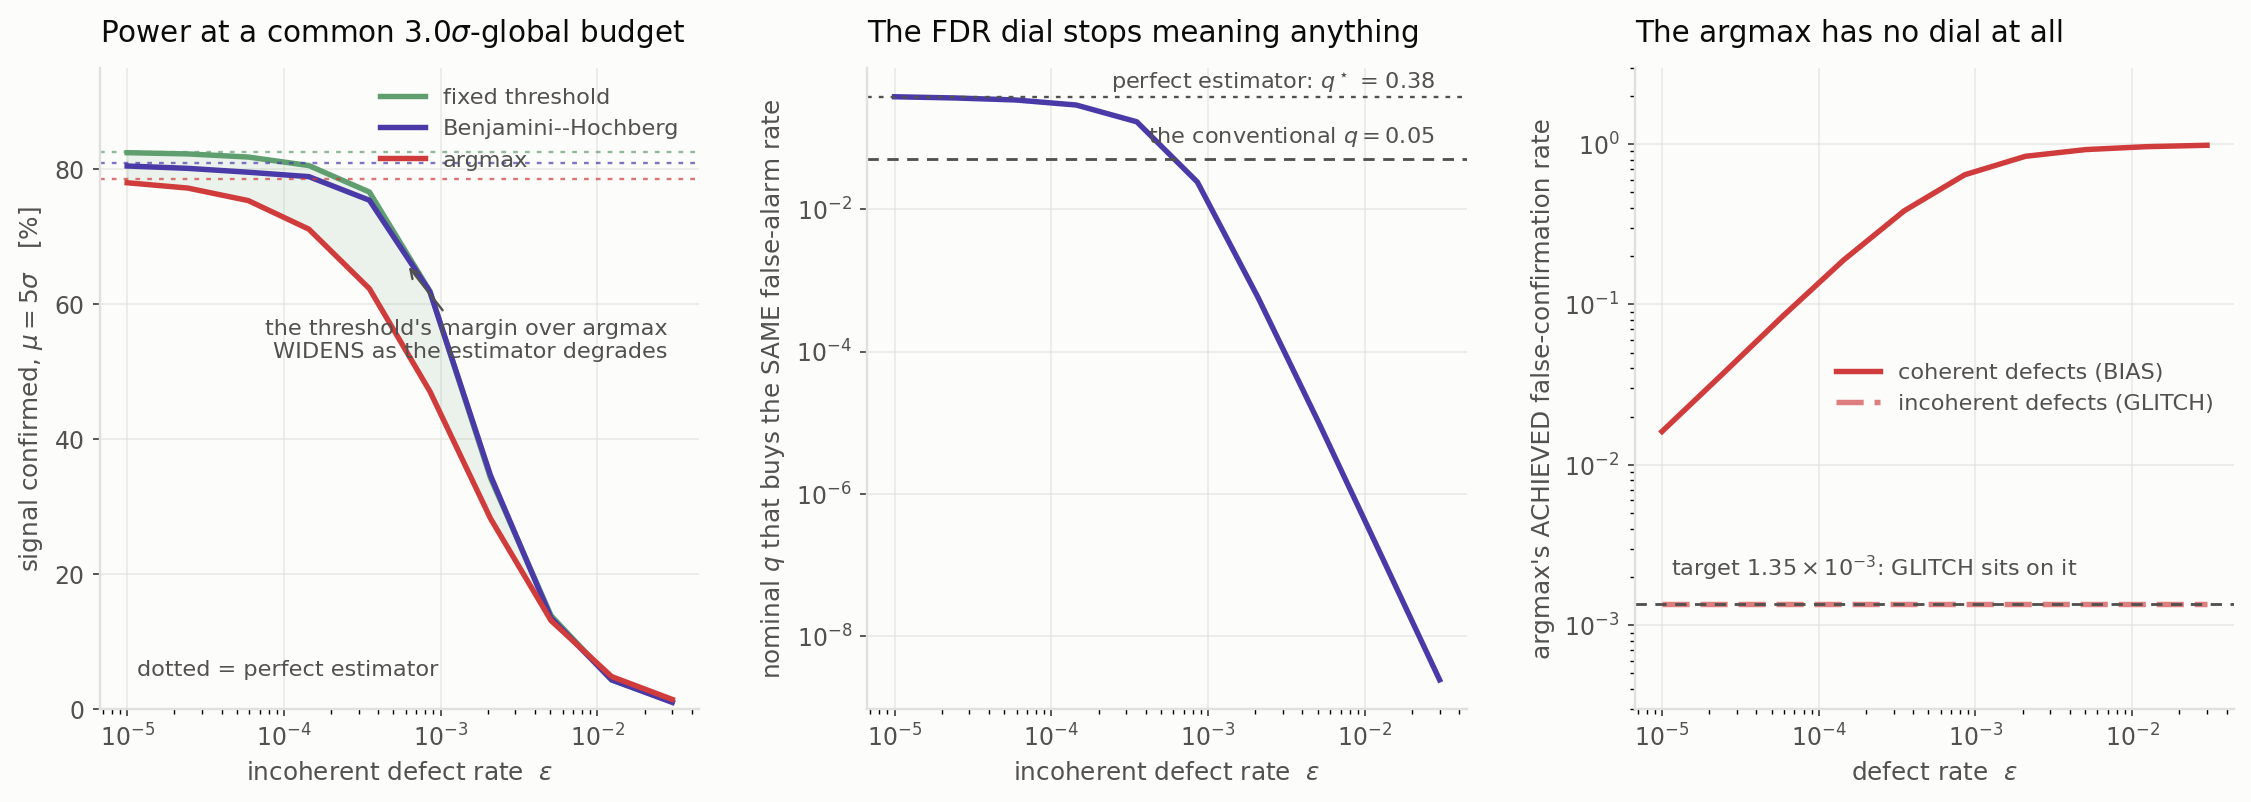
\includegraphics[width=\textwidth]{bh_outliers.png}
\caption{\textbf{Left:} confirmation probability for a $5\sigma$ signal as the estimator degrades,
all three rules held at the same false-alarm budget; dotted lines are the perfect-estimator
values. \textbf{Middle:} the nominal FDR that buys that budget, against the conventional $q=0.05$.
\textbf{Right:} the argmax's achieved false-alarm rate, which it has no parameter to control.}
\label{fig:selnoise}
\end{figure}

The last row of Table~\ref{tab:selnoise} is the same result as Section~\ref{sec:abnoise} seen from
a different direction: a coherent defect is indistinguishable from a signal, so no selection rule
can help against it. The threshold remains formally calibratable --- it can always be raised, and
its reachable floor is $10^{-9}$ against BH's $2.5\times10^{-3}$ --- but only at essentially zero
power. That is a background-modelling problem, not a selection-rule problem.

Two caveats. The bins here are independent, where a real scan has correlated neighbouring mass
bins; and the defect magnitude is fixed at $2\sigma$, so the size of the gaps scales with it while
the ordering does not. At the heaviest incoherent contamination all three rules are equally dead
and the argmax nominally edges ahead by a few tenths of a point, which is not a meaningful
ranking.

\subsection{What this implies for a data-directed scan}

\begin{enumerate}[leftmargin=1.6em,itemsep=3pt]
  \item \textbf{Do not select by rank alone.} ``Take the most significant bin'' is a dominated
strategy. Selecting on absolute significance recovers the information the ranking throws away, at
identical false-alarm cost, and gains a few percentage points of power at every signal strength.
With an imperfect estimator the argument gets stronger rather than weaker
(Section~\ref{sec:selnoise}): the margin grows to more than ten points, and the argmax loses
control of its false-alarm rate entirely.
  \item \textbf{Fix the fake budget, not the threshold.} The natural, scan-size-independent
        statement of an operating point is ``one expected background candidate per experiment'',
        which determines $t^\star$ from $n$. Quoting a bare $z$ threshold hides the scan size.
  \item \textbf{An FDR rule is a defensible middle ground, but never quote the nominal $q$ as a
false-alarm specification.} BH costs a little power relative to the matched threshold, and it
comes with a guarantee that is easy to state to a reviewer. What that guarantee does not survive
is a miscalibrated tail: the $q$ needed to buy a given false-alarm rate moves by six orders of
magnitude across the contamination range of Section~\ref{sec:selnoise}, and under coherent defects
no $q$ buys it. Whichever rule is adopted, calibrate and quote the \emph{achieved} rate.
  \item \textbf{The confirmation stage is cheap and carries no trials factor.} That is the
        structural fact the next section is built on.
\end{enumerate}

\section{Two-stage A/B unblinding}
\label{sec:ab}

\subsection{The proposal}

Split the dataset into a fraction $f$ (sample A, exploration) and $1-f$ (sample B, confirmation).
Scan \emph{everything} in A with \emph{no} global correction, since what happens in A is selection
rather than inference. Pre-register every window with local $Z_A \ge Z_{\mathrm{cut}}$. Unblind
only those windows in B, and make the discovery claim on the B-only $p$-value, corrected for the
$k$ pre-registered windows.

The attraction is immediate. The trials factor in B is not modelled but \emph{counted}: it is the
number of lines in a frozen document. For a classical fixed-window search that is a modest
convenience. For a neural-network-driven scan, where ``how many independent looks did the network
take'' has no crisp answer, it is the difference between a defensible number and an argument.

\subsection{The cost}

Nothing is free, and here the trade is explicit. One avoids a logarithmic penalty by giving up
luminosity, which costs $\sqrt{f}$ on the significance. For a signal whose full-dataset
local significance would be $Z_{\mathrm{full}}$, the two stages fluctuate independently, so the
joint discovery probability is
\begin{equation}
  P_{\mathrm{disc}}
  \;=\;
  \Phi\!\left(\sqrt{f}\,Z_{\mathrm{full}} - Z_{\mathrm{cut}}\right)
  \cdot
  \Phi\!\left(\sqrt{1-f}\,Z_{\mathrm{full}} - Z_{B}^{\mathrm{req}}\right),
  \qquad
  Z_B^{\mathrm{req}} = \sqrt{25 + 2\ln k_{\mathrm{eff}}},
  \label{eq:abpower}
\end{equation}
with $k_{\mathrm{eff}} = N\,p_1(Z_{\mathrm{cut}}) + 1$ the expected number of pre-registered
windows. The reach is the $Z_{\mathrm{full}}$ at which $P_{\mathrm{disc}} = 50\,\%$.

The distinction between joint power and the naive median arithmetic matters. Requiring each stage
to succeed at its median gives $Z_{\mathrm{med}} = \max(Z_{\mathrm{cut}}/\sqrt{f},\,
Z_B^{\mathrm{req}}/\sqrt{1-f})$, which \emph{underestimates} the required signal wherever both
constraints bind, since two independent coin flips at 50\,\% each give 25\,\% jointly.
Equation~\eqref{eq:abpower} is the honest figure of merit, and toy Monte Carlo reproduces it to
$0.03\sigma$.

At this study's budget ($N = 6616$, single-stage reach $6.53\sigma$):

\begin{table}[htbp]
\centering
\caption{Signal strength required for a 50\,\% probability of discovery, as a function of the
splitting scheme, at $N = 6616$ independent looks.}
\label{tab:abcost}
\begin{tabular}{lrr}
\toprule
procedure & reach $Z_{\mathrm{full}}$ & cost \\
\midrule
single-stage full scan, exactly corrected & 6.53 & --- \\
optimised split ($f \approx 0.2$--$0.3$, $Z_{\mathrm{cut}} \approx 2$--$3$) & $\sim7.0$ & $+0.5\sigma$ \\
naive 50/50 split, $Z_{\mathrm{cut}} = 3$ & $\sim8.0$ & $+1.4\sigma$ \\
\bottomrule
\end{tabular}
\end{table}

\begin{figure}[htbp]
\centering
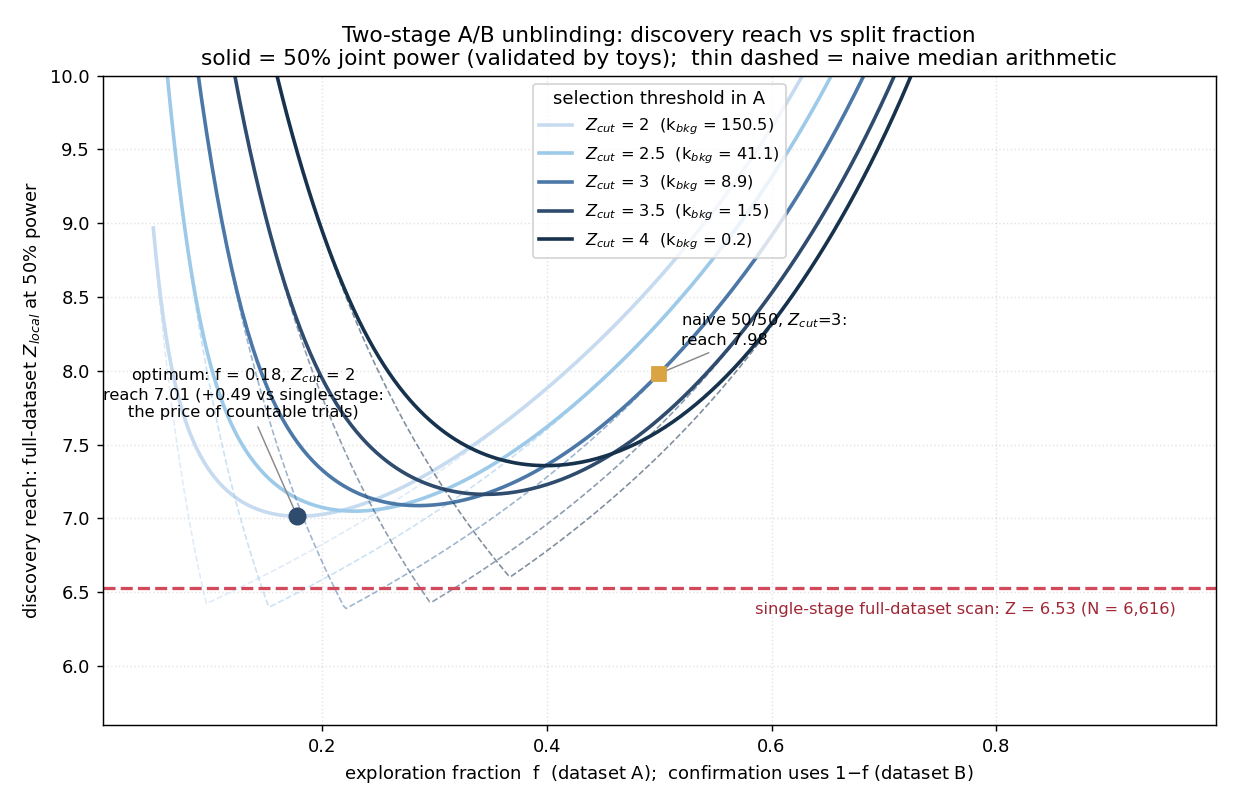
\includegraphics[width=0.9\textwidth]{ab_split_reach.png}
\caption{Discovery reach versus exploration fraction $f$, for several stage-1 selection thresholds.
Solid curves are 50\,\% joint power (Eq.~\eqref{eq:abpower}), thin dashed the naive median
arithmetic. The red line is the exactly corrected single-stage scan. The optimum is markedly asymmetric, with a small exploration sample and a large confirmation
sample, and the naive 50/50 split is a poor choice.}
\label{fig:abreach}
\end{figure}

\subsection{The look-elsewhere effect is conserved, not reduced}
\label{sec:abcons}

It is tempting to expect a trials count large enough to make splitting pay. There is none, and the
reason is an identity rather than a numerical accident. The cost $2\ln N$ factorises:
\begin{equation*}
  2\ln N \;=\; 2\ln\!\frac{N}{k} \;+\; 2\ln k,
\end{equation*}
where the first term is paid implicitly, as the stage-1 selection cut that reduces $N$ looks to
$k$ pre-registered windows, and the second explicitly in B. Splitting \emph{relocates} the penalty
rather than removing it. What remains is the two-coin penalty, the requirement that both
independent halves succeed, which runs from $+0.3$ to $+0.5\sigma$ between $N = 10$ and $N =
10^{10}$ and never crosses zero.

The number of unblinded windows barely matters: moving $k$ from 1 to 1000 changes the reach by
$0.15\sigma$, so $k$ can be chosen on practical grounds ($k \approx 10$).

\begin{figure}[htbp]
\centering
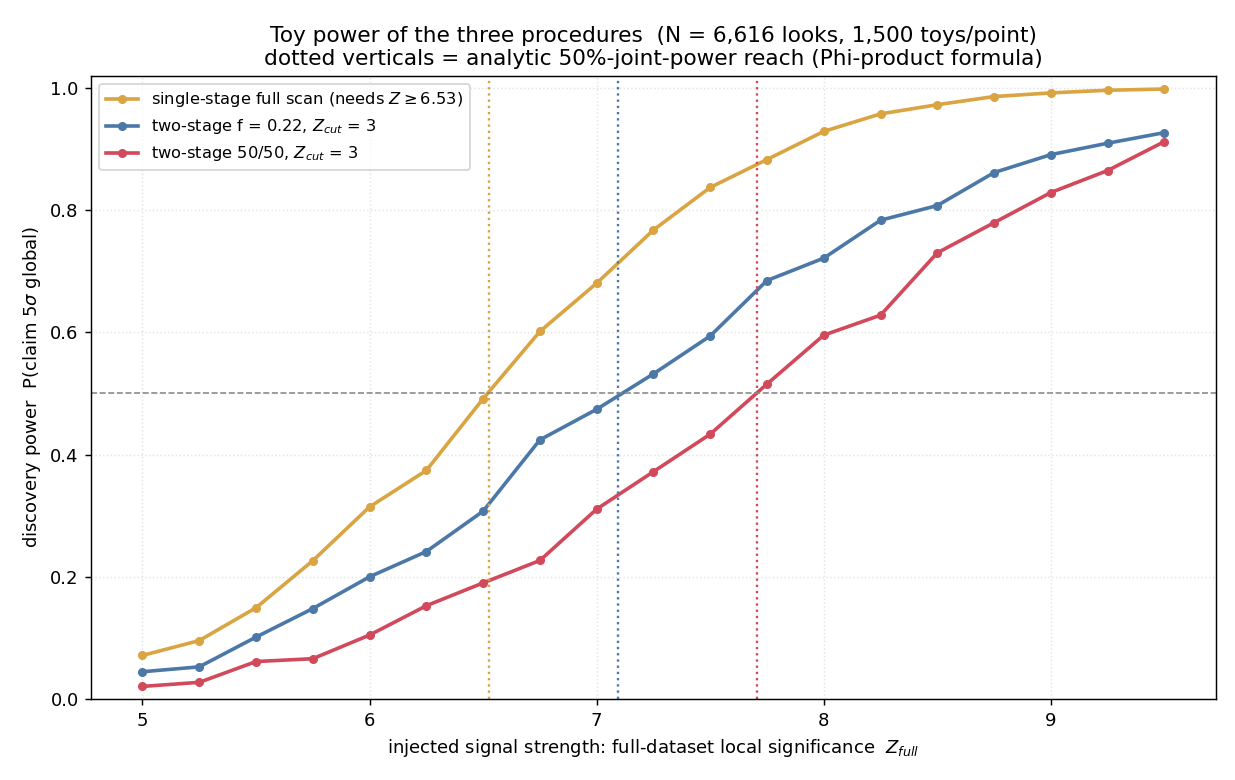
\includegraphics[width=0.92\textwidth]{ab_toys_power.png}
\caption{Toy Monte-Carlo validation: discovery power versus injected signal strength for the three
procedures, with the analytic median-reach values as vertical lines. The toys treat the budget's
$N$ effective looks as independent standard normals under background-only and recover the
full-dataset scan exactly as $z_{\mathrm{full}} = \sqrt{f}z_A + \sqrt{1-f}z_B$.}
\label{fig:abtoys}
\end{figure}

\subsection{Would swapping the halves recover it?}
\label{sec:abswap}

The natural objection to that identity is that half the luminosity sits idle at each stage. Why
not run \emph{both} directions --- explore in A and confirm in B, \emph{and} explore in B and
confirm in A --- and claim if either confirms? This is two-fold cross-validation of the
\emph{claim}, and it is a genuinely different procedure rather than a relabelling.

The trade is explicit. Both directions pre-register, so the confirmation windows double,
$k \to 2k$, costing $2\ln 2$ on the B bar: at $Z_{\mathrm{cut}} = 3$ and $N = 6616$,
$Z_B^{\mathrm{req}}$ moves from $5.64$ to $5.75$. What is bought is a second chance at the same
signal. Since $Z_B^{\mathrm{req}} > Z_{\mathrm{cut}}$, the two directions coincide only where
\emph{both} halves clear the claim bar, so the union power is
\begin{equation}
  P^{\mathrm{sym}}_{\mathrm{disc}}
  \;=\;
  \Phi^{A}_{\mathrm{cut}}\Phi^{B}_{\mathrm{req}}
  \;+\;
  \Phi^{B}_{\mathrm{cut}}\Phi^{A}_{\mathrm{req}}
  \;-\;
  \Phi^{A}_{\mathrm{req}}\Phi^{B}_{\mathrm{req}},
  \qquad
  \Phi^{A}_{x} = \Phi\!\left(\sqrt{f}\,Z_{\mathrm{full}} - Z_{x}\right),
  \label{eq:abswap}
\end{equation}
and $\Phi^{B}_{x}$ the same with $f \to 1-f$; toys reproduce it to $0.01\sigma$. At fixed
thresholds the gain over one direction is a factor
$2 - \Phi_{\mathrm{req}}/\Phi_{\mathrm{cut}}$, that is, at most two.

That gain is collected only when both directions have comparable power, which means $f = 1/2$ ---
and $f = 1/2$ is precisely the split the one-way analysis rejects, because confirmation is the
luminosity-hungry stage. The swap therefore does not beat the asymmetric scheme; it
\emph{rescues the symmetric one}.

\begin{table}[htbp]
\centering
\caption{One-way splitting against the symmetrised swap at $N = 6616$ (single-stage reach
$6.53$). The first two rows re-optimise $f$ at fixed $Z_{\mathrm{cut}}$; the last optimises
$(f, Z_{\mathrm{cut}})$ inside the practical design box $Z_{\mathrm{cut}} = 2$--$4.5$.}
\label{tab:abswap}
\begin{tabular}{lrrrr}
\toprule
 & \multicolumn{2}{c}{one-way} & \multicolumn{2}{c}{swapped} \\
\cmidrule(lr){2-3}\cmidrule(lr){4-5}
design & reach & cost & reach & cost \\
\midrule
$50/50$, $Z_{\mathrm{cut}} = 3$ & 7.98 & $+1.45$ & \textbf{7.38} & $\mathbf{+0.86}$ \\
$f = 0.30$, $Z_{\mathrm{cut}} = 3$ (recommended) & \textbf{7.09} & $\mathbf{+0.56}$ & 7.15 & $+0.63$ \\
best design in the practical box & \textbf{7.01} & $\mathbf{+0.49}$ & 7.03 & $+0.51$ \\
\bottomrule
\end{tabular}
\end{table}

Applied on top of the recommended working point the swap is actively harmful: the second
direction would have to confirm a $5\sigma$-global result on $30\%$ of the data, so it almost
never fires, and one pays the $2\ln 2$ for a dead direction. Optimised freely inside the
practical box the two schemes are a wash, $+0.49\sigma$ against $+0.51\sigma$, and the gap stays
within $0.11\sigma$ over nine decades of $N$, changing sign with the design box rather than
crossing over at any particular trials count.

Why neither can win is clearest geometrically. In the $(z_A, z_B)$ plane the Neyman--Pearson
acceptance region for a mean shift is the half-plane
$\sqrt{f}\,z_A + \sqrt{1-f}\,z_B > \sqrt{25 + 2\ln N}$ --- which is exactly the single-stage scan
on the recombined dataset. One-way splitting approximates that half-plane with an $L$-shaped
corner, the swap with a two-step staircase. More steps track the line more closely, which is why
the swap repairs the $50/50$ split, but every step multiplies the pre-registered windows.
Conservation of the look-elsewhere effect is that staircase-versus-half-plane inefficiency, and no
number of folds removes it.

The decisive objection, though, is not statistical. Of the three things the split buys
(Section~\ref{sec:abwhy}) the swap keeps two and destroys the third. The trials factor is still
counted and still auditable --- $2k$ is as countable as $k$ --- but procedural blindness is gone:
after the first direction the analyst has seen B, so the second direction's ``confirmation'' on A
is made by someone who already knows both halves. It is valid only if the entire two-directional
procedure is frozen and executed in a single automated pass, and a review committee is entitled to
discount it even then. The swap also does nothing about the correlated-systematics mode of
Section~\ref{sec:abblind}, which for a data-directed analysis is the leading one.

None of this argues against symmetrising the \emph{training}, which is a separate question taken
up in Section~\ref{sec:abnoise}: holding the background model out of the sample it scores is nearly
free and attacks the sculpting mode directly. Symmetrising the \emph{claim} is the thing that
costs, and on this budget it buys nothing.

\subsection{When the split is nonetheless the right choice}
\label{sec:abwhy}

The split wins if and only if the single-stage trials factor one would have to \emph{defend}
exceeds $R^\star \approx 13$ times the true $N$. For a classical fixed-window scan that is
implausible, and the corrected single stage wins outright. For a network-driven hunt a factor of
13 in forced conservatism is entirely imaginable, and that, rather than the logarithm, is the
quantitative case for two-stage unblinding. It buys three things:

\begin{itemize}[leftmargin=1.4em,itemsep=2pt]
  \item an \textbf{exactly countable} trials factor in B,
  \item \textbf{auditability}: the correction is the number of lines in a document frozen before
        unblinding, and
  \item \textbf{procedural blindness}: the analysis cannot be tuned on the confirmation sample.
\end{itemize}

\subsection{The failure mode splitting does \emph{not} address}
\label{sec:abblind}

A/B splitting attacks the \emph{statistical} look-elsewhere effect only. A spurious bump caused by
correlated systematics, such as background mis-modelling or a network that has learnt to sculpt a
peak, appears identically in both halves and will happily ``confirm''. For a data-directed
analysis this is not a corner case but the leading failure mode. The split protects against
fluctuations, not against the analysis fooling itself. That statement is exact but incomplete:
between a pure fluctuation and a fully correlated systematic lies everything an imperfect
estimator does, and Section~\ref{sec:abnoise} prices the split over that range.

\subsection{What changes if the significance estimator is imperfect}
\label{sec:abnoise}

Everything above assumes a perfectly calibrated estimator: every look returns $Z \sim N(0,1)$
under background, so the only thing to control is the look-elsewhere effect, and splitting can
only lose. A network-driven scan does not have that estimator. It has one that occasionally
returns an outlier --- a fit that failed to converge on this subsample, a background model that
has absorbed a fluctuation, a window where the shape is simply wrong. Repricing the split against
that estimator changes the verdict, and the reason it changes is worth more than the number.

The only property of an outlier that an A/B split can see is whether it \emph{repeats in the other
half}. That suggests three classes, distinguished by nothing but their correlation across the
split:

\begin{table}[htbp]
\centering
\caption{Classes of estimator defect, by how they correlate between the two halves. Only the last
column matters to a split.}
\label{tab:abdefect}
\begin{tabular}{lp{4.5cm}p{5.4cm}}
\toprule
class & physical origin & behaviour across the split \\
\midrule
\textsc{bias} & mismodelled background or detector artefact in that window &
  the pull is $\delta B/\sqrt{B} = \delta\sqrt{wB}$, so it grows with luminosity exactly like a
  signal and is \textbf{identical} in both halves \\
\textsc{var} & the look's uncertainty is underestimated by a factor $s$ &
  the miscalibration is shared, but what it amplifies is each half's \emph{independent}
  fluctuation \\
\textsc{glitch} & a per-\emph{run} failure: non-convergence on this subsample, a network
  artefact, a corrupted input &
  redrawn \textbf{independently} every time the estimator is run \\
\bottomrule
\end{tabular}
\end{table}

The mechanism is a one-line geometric statement, and Fig.~\ref{fig:abmech} is the whole section in
a picture. In the $(Z_A, Z_B)$ plane a coherent pull $b$ places a look at
$(\sqrt{f}\,b,\,\sqrt{1-f}\,b)$ --- on the locus $Z_B = \sqrt{(1-f)/f}\,Z_A$, which is precisely
where a real signal of the same strength sits. An incoherent one places it near the $Z_B \approx 0$
axis. The split is a cut that separates the axis from the locus, and by construction cannot
separate the locus from itself. It follows immediately that a coherent defect is not merely hard
for the split to reject: it is \emph{exactly as confirmable as a signal}, which is the content of
Section~\ref{sec:abblind} restated.

\begin{figure}[htbp]
\centering
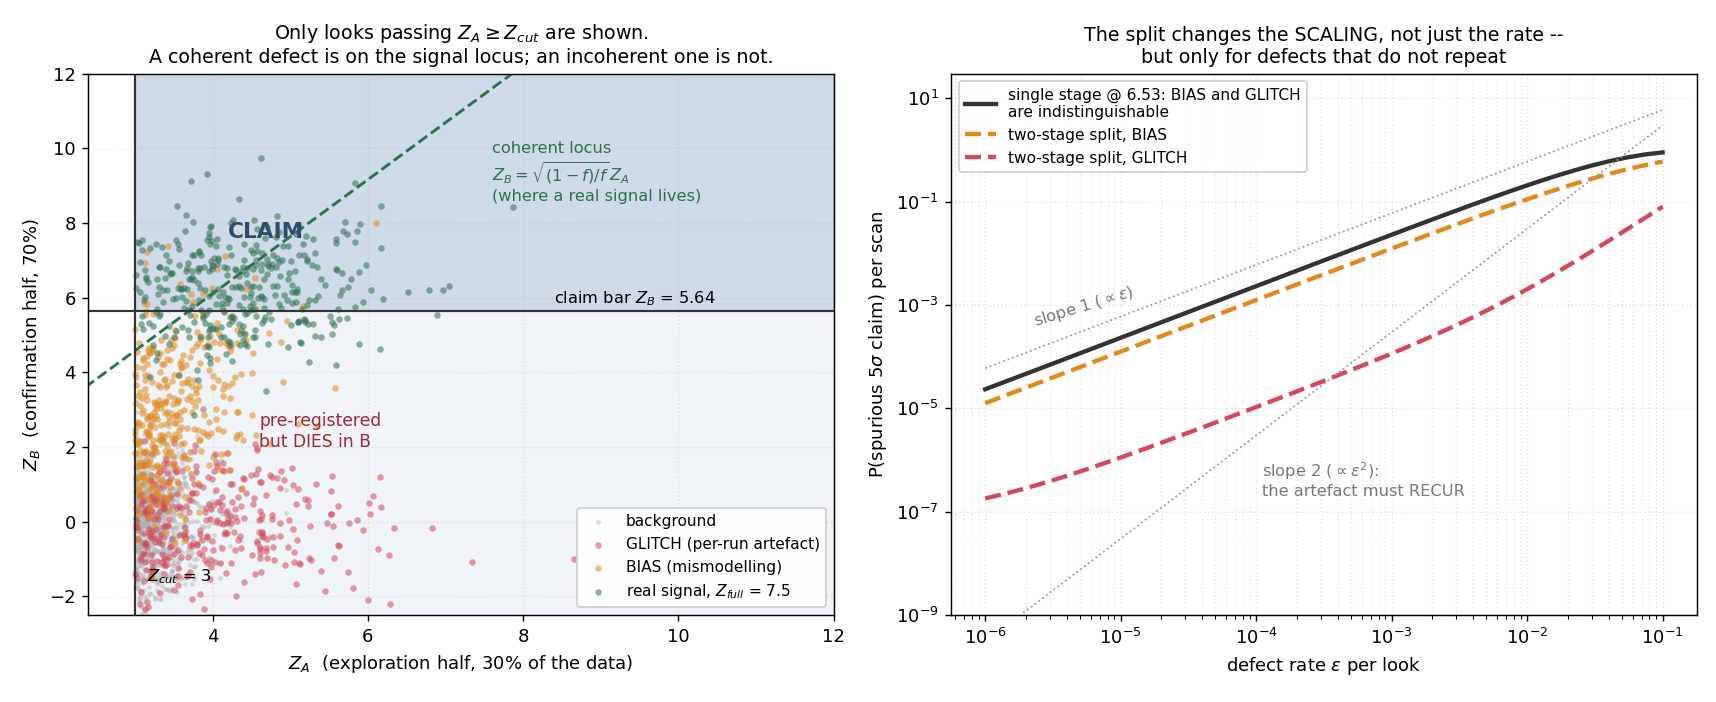
\includegraphics[width=\textwidth]{ab_outliers_mechanism.png}
\caption{\textbf{Left:} looks that pass the stage-1 cut, in the plane of the two half-dataset
significances. Real signals and coherent mismodellings populate the same locus; per-run artefacts
sit on the $Z_B \approx 0$ axis and die at the claim bar. \textbf{Right:} the resulting
spurious-claim rate. The two defects are \emph{identical} to a single-stage scan --- one curve, by
construction --- and the split separates them by changing the scaling from $\epsilon$ to
$\epsilon^{2}$ for the incoherent one alone.}
\label{fig:abmech}
\end{figure}

The same two failure modes on an actual falling spectrum are shown in Fig.~\ref{fig:abspec}: a
background fit that undershoots by $\sim10\,\%$ in the A half alone produces a $4.1\sigma$
excess that is duly pre-registered and then collapses to $2.6\sigma$ in B, while a background
genuinely mismodelled by $8.8\,\%$ gives $4.2\sigma$ in A and $6.9\sigma$ in B and clears the claim
bar.

\begin{figure}[htbp]
\centering
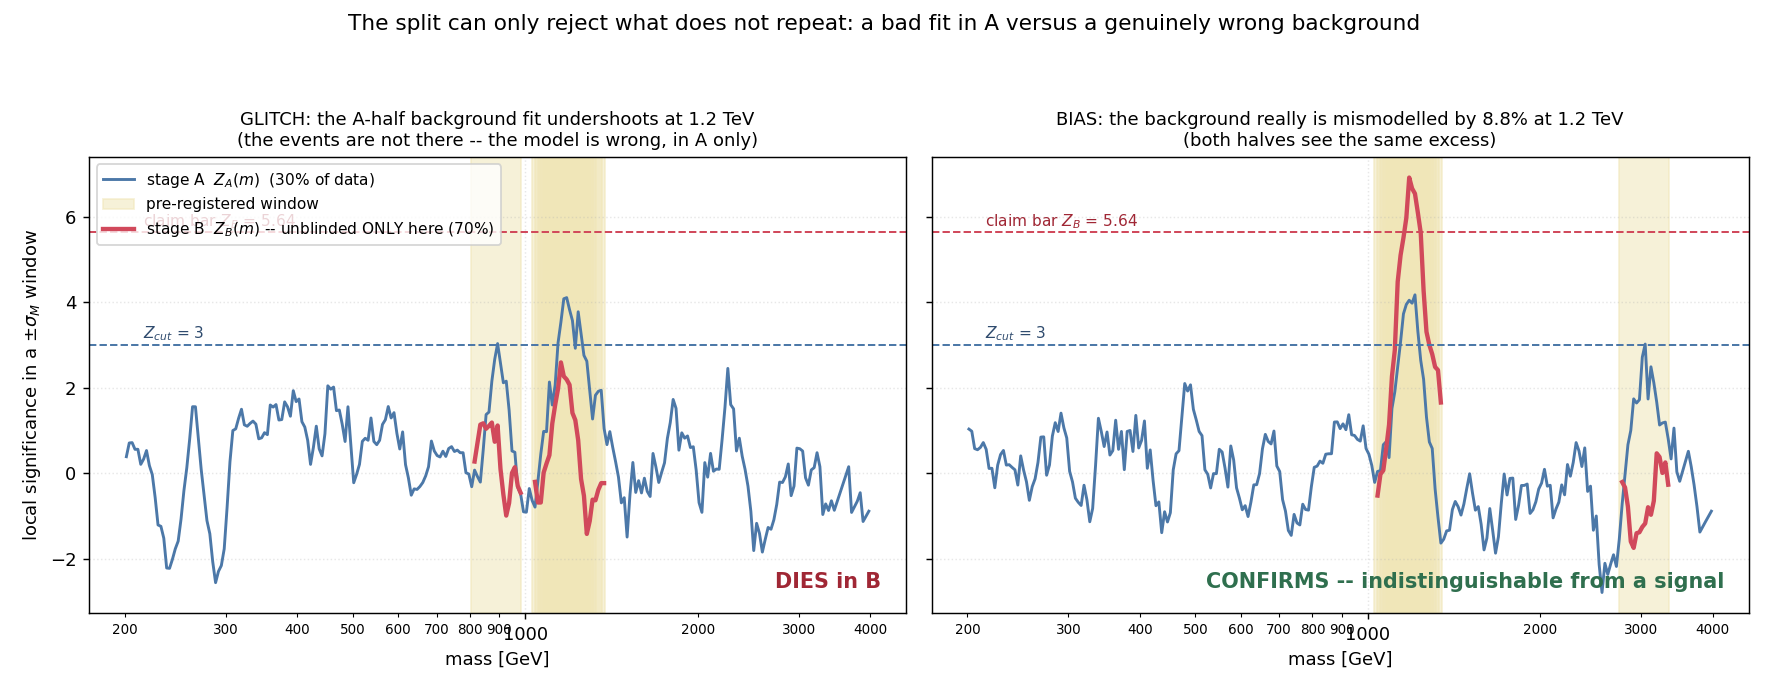
\includegraphics[width=\textwidth]{ab_outliers_spectrum.png}
\caption{Toy spectra scored the way an analysis would score them, at the recommended working point.
\textbf{Left:} the A-half background model is locally wrong, so the excess exists only in the
estimator and stage B removes it. \textbf{Right:} the background model is wrong for both halves, so
the excess is real in the data and confirms. Only the first of these is a fluctuation in the sense
the split can act on.}
\label{fig:abspec}
\end{figure}

The comparison cannot be made on raw false-alarm rates, because the single stage can always buy
robustness by raising its bar. The honest figure of merit is therefore \emph{matched}: raise the
single-stage threshold until it is equally likely to make a spurious claim, and only then compare
reach. Table~\ref{tab:abnoise} does this at the recommended working point, with each defect
occurring at rate $\epsilon = 10^{-3}$ and magnitude $\sim2\sigma$.

\begin{table}[htbp]
\centering
\caption{Matched-robustness comparison at $f = 0.30$, $Z_{\mathrm{cut}} = 3$, $N = 6616$, for a
defect rate $\epsilon = 10^{-3}$ ($\approx 1$ artefact above $3\sigma$ per scan). A positive gain
means the split reaches a \emph{weaker} signal than a single-stage scan that is equally safe.}
\label{tab:abnoise}
\begin{tabular}{lrrrr}
\toprule
estimator & suppression & split reach & matched bar & gain \\
\midrule
perfect (the assumption above) & --- & 7.09 & 6.53 & $-0.56\sigma$ \\
\textsc{bias} & $1.9\times$ & 7.08 & 6.95 & $-0.14\sigma$ \\
\textsc{var} ($s = 2$) & $3.5\times$ & 7.10 & 7.20 & $+0.10\sigma$ \\
\textsc{glitch} & $199\times$ & 7.11 & \textbf{9.61} & $\mathbf{+2.50\sigma}$ \\
\bottomrule
\end{tabular}
\end{table}

Against a per-run glitch the split suppresses the spurious-claim rate by two orders of magnitude,
because the artefact must recur \emph{independently} in B above $5.6$: the rate goes as
$\epsilon^2$ rather than $\epsilon$. A single-stage scan would have to demand $Z \ge 9.6$ to be as
safe. Against a coherent bias the split suppresses by $1.9\times$, but that is not discrimination
--- it is merely the split's own worse reach hurting fakes along with signal --- and the single
stage buys the same factor for $+0.42\sigma$, which is cheaper than the split costs. Section
\ref{sec:abblind} is the $\rho = 1$ limit of this table.

\subsubsection*{Coherence is the deciding variable}

Interpolating between the two extremes with a coherent fraction $\rho$ (Fig.~\ref{fig:abnoise}),
the break-even sits at $\rho^\star \approx 0.80$ and moves by less than $0.02$ over two decades in
the overall defect rate. The rule is therefore unusually portable:

\begin{quote}
\textbf{If fewer than about four in five of the estimator's outliers repeat in the other half, the
split pays for itself.}
\end{quote}

Under a plausible cocktail --- coherent bias, bad fits and glitches each at $10^{-3}$, together
$\approx 3$ artefacts above $3\sigma$ per scan --- the net is $+0.29\sigma$ in the split's favour,
against $-0.56\sigma$ for a perfect estimator. And $\rho$ is measurable \emph{before} unblinding:
split the sidebands or MC-only pseudo-data, and count what fraction of the $3\sigma$ excesses
recurs.

\begin{figure}[htbp]
\centering
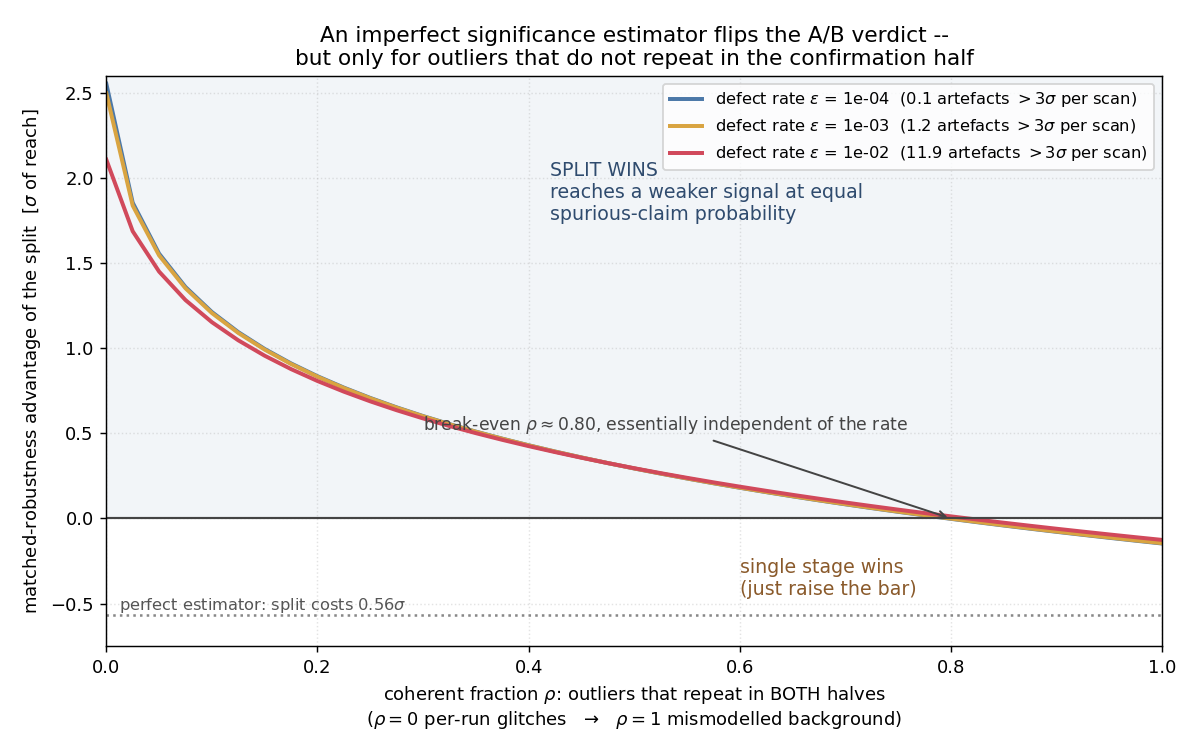
\includegraphics[width=0.92\textwidth]{ab_split_outliers.png}
\caption{Matched-robustness advantage of the split as a function of the coherent fraction $\rho$
of the estimator's outliers, at three defect rates. The dotted line is the pure cost of splitting
with a perfect estimator. The break-even is essentially rate-independent, so the criterion is a
property of the estimator's failure modes rather than of how often they occur.}
\label{fig:abnoise}
\end{figure}

\subsubsection*{Where the training arrangement enters}

The sharpest case is a background model \emph{fit to data}, which is the data-directed situation.
Fitting it on the same events one then tests for excesses is overfitting, and overfitting is a
\textsc{glitch}-type defect tied to the specific events in that half. A single pass cannot escape
it: there is no held-out half. Three arrangements are available to a split, and they are not
equivalent:

\begin{enumerate}[leftmargin=1.6em,itemsep=3pt]
  \item \textbf{self-contained} --- train on A and score A, train on B and score B. Both stages
        overfit, but independently, so the claim is $\epsilon^2$-suppressed. Bookkeeping exact.
        Worth $+2.50\sigma$.
  \item \textbf{full cross} --- train on B and score A, train on A and score B. No overfitting
        anywhere, worth $+5.67\sigma$, \emph{but} the stage-A selection is now a function of B
        through the trained model, so the pre-registration is no longer independent of the
        confirmation sample and the $k$-coin $p$-value is no longer exact.
  \item \textbf{A-trained throughout} --- train on A, score A to select, then apply that same
        frozen model to B. The confirmation $Z$ is produced by an estimator that has never seen a
        single B event, so overfitting is removed \emph{by construction} rather than beaten down
        statistically; and nothing about B enters the pre-registration, so the bookkeeping stays
        exact. Worth $+5.64\sigma$.
\end{enumerate}

Arrangement 3 dominates: it recovers all but $0.03\sigma$ of the full-cross gain while keeping the
blindness that made the scheme worth adopting. The reason it can is that the overfitting it leaves
in place --- in stage A --- only inflates the candidate list ($k$: $8.9 \to 10.1$), and $k$ enters
the bar as $2\ln k$. \textbf{Contaminating the exploration stage is logarithmically cheap;
contaminating the confirmation stage is what costs.}

\subsubsection*{Two caveats on this result}

Part of the \textsc{glitch} gain is available without splitting. If the artefact is purely
seed- or initialisation-dependent, re-running the estimator with different seeds on the
\emph{same} data catches it at no cost in reach. What a seed jackknife cannot decorrelate is a
defect tied to a specific \emph{data} fluctuation --- overfitting, or a fit driven by the actual
events in that window. Only a data split touches those, which is exactly the data-directed failure
mode, so the claim is narrower than the raw $+2.5\sigma$ but lands on the case at hand.

Second, and more important: after the split the residual spurious rate is essentially
\emph{entirely} coherent. The glitch and variance components contribute $0.9\,\%$ and $0.1\,\%$ of
what still gets through. The split does not make the analysis safe --- it changes what one has to
worry about, from ``is my estimator glitchy?'' to ``is my background model wrong in that window?''.
That residual has to be controlled by other means (validation regions, spurious-signal tests,
alternative background parameterisations), because the confirmation stage will endorse a
mismodelled background as enthusiastically as a real signal.

The overall repricing is then a change of argument rather than of arithmetic.
Section~\ref{sec:abcons} stands exactly as written: with a perfect estimator, splitting relocates
the look-elsewhere effect and cannot reduce it. But that was answering the wrong question for a
data-directed search. The split is not a look-elsewhere device --- it is an
\textbf{estimator-robustness device}, and priced as one, $0.5\sigma$ is cheap.

\subsection{Recommended working point}

If the scheme is adopted, the design that follows from the above is:

\begin{itemize}[leftmargin=1.4em,itemsep=2pt]
  \item exploration fraction $f \approx 0.25$--$0.35$, stage-1 threshold $Z_{\mathrm{cut}} = 3$
        (giving $\approx 9$ pre-registered windows at this budget);
  \item pre-registered $\pm2\sigma_M$ windows, with the outcome ladder written down before
        unblinding;
  \item the background model \textbf{trained on A alone} and applied frozen to B
        (arrangement 3 of Section~\ref{sec:abnoise}), so that the confirmation significance comes
        from an estimator that has never seen a B event, without leaking B into the
        pre-registration;
  \item the claim quoted as a \textbf{global} significance over the pre-registered windows:
        evidence at $Z_B^{\mathrm{global}} \ge 3$ (local $Z_B \ge 4.0$), discovery at
        $Z_B^{\mathrm{global}} \ge 5$ (local $5.6$). The false-evidence rate per opening is then
        $1.35\times10^{-3}$ by construction, whatever number of windows A flags;
  \item B alone for the claim $p$-value, A$+$B for the measurement.
\end{itemize}

\section{Software and reproducibility}
\label{sec:software}

Every number, table and figure in this note is produced by code in the accompanying repository, and
the intention is that a reader can regenerate any of them rather than take them on trust. Nothing
in the chain reads an experiment-internal input, so ``regenerate'' means from a clone and nothing
else.

\subsection{The two modules everything rests on}

The whole budget derives from two data-free modules, and keeping them small and singular is what
makes the claim checkable:

\begin{itemize}[leftmargin=1.4em,itemsep=2pt]
  \item \code{scripts/bump\_observables.py} --- the bump observables with their fractional
resolutions, analyzable floors and published scan windows, each window carrying a per-channel
source note (Appendix~\ref{app:windows}). It also owns the two structural maps that decide what
counts as one spectrum: the same-axis merges and the lepton-flavour split. It is imported, never
duplicated; a floor or a window redefined in a consumer would be a bug.
  \item \code{scripts/public\_obs\_map.py} --- the map from public BSM model classes onto the spectra
they populate, plus the published event-selection multiplicity per spectrum.
\end{itemize}

Both carry import-time assertions that keep the flavour layer complete: every leaf channel must have
a window and a floor, and no flavour-inclusive parent may keep one, which is what prevents a channel
being counted both as itself and as part of its parent.

\subsection{Layout and rebuilding}

\begin{itemize}[leftmargin=1.4em,itemsep=2pt]
  \item \code{scripts/}, the pipeline, one concern per file.
  \item \code{results/tables/}, machine-readable output, including the cached Monte Carlo of
Section~\ref{sec:selection}.
  \item \code{results/plots/}, the figures of this note.
  \item \code{results/overviews/}, the long-form reports the sections here condense.
  \item \code{docs/}, holding \code{METHOD\_NOTES.md} (conventions and the reasoning behind the
counting choices), \code{OUTPUTS.md} (every output file mapped to the script that writes it), and
this note.
\end{itemize}

The pipeline is driven by a single makefile whose targets are real files with real prerequisites,
so a rerun redoes only what is stale:

\begin{verbatim}
    pip install -r requirements.txt   # numpy, scipy, matplotlib
    make all                          # budget + ab + stats
    make help                         # the individual stages
\end{verbatim}

The stages are \code{budget} (Sections~\ref{sec:budget} to~\ref{sec:excess}), \code{ab}
(Section~\ref{sec:ab}) and \code{stats} (Section~\ref{sec:selection}). The budget itself uses only
the Python standard library; \code{ab} and \code{stats} need NumPy~\cite{numpy},
SciPy~\cite{scipy} and Matplotlib~\cite{matplotlib}.

\subsection{Determinism}

All Monte Carlo is explicitly seeded, and rebuilding the figure set reproduces the committed files
byte for byte. That is worth more than it sounds, because it means a changed figure signals that an
input or a method changed rather than that a random seed moved. The two genuinely slow computations,
the Benjamini--Hochberg $q$ scan and its imperfect-estimator variant, are cached as \code{.npz}
files and rerun only on request.

\subsection{Relation to the catalogue note}

One question is deliberately absent here: which of these 46 spectra a given collaboration has
actually produced signal samples for. That is a statement about a production program rather than
about the search budget, it cannot be made from public information, and answering it does not change
any number in this note --- the windows are published-search windows either way. It is treated in a
companion ATLAS-internal note, which imports the two modules above unchanged so that the two
documents cannot drift apart on what a spectrum is.

\section{Summary and recommendations}
\label{sec:summary}

\subsection{What was established}

\begin{enumerate}[leftmargin=1.6em,itemsep=4pt]
  \item \textbf{Models collapse onto spectra.} Classified by \emph{where the bump appears} rather
than by theory, and with lepton flavour and $b$-tag content counted as part of the mass axis, the
public BSM resonance model classes map onto \textbf{46 canonical spectra}. The number of searches is
set by the number of spectra, not by the number of models.
  \item \textbf{The search budget.} $\Nsig \approx 3.7\times10^{3}$ inclusively,
        $6.6\times10^{3}$ at realistic event-selection granularity, hence $\Zloc \approx 6.4$ to
$6.5$ for a $5\sigma$ global discovery, stable to $\pm0.1\sigma$ against every counting choice
varied. \textbf{Covering the entire known BSM resonance space costs about one extra unit of $\sigma$
over a single counting experiment.}
  \item \textbf{The combinatorial scan costs half a sigma more.} 150 exclusive object categories
        and 1094 mass groups give $\Nsig = 1.4\times10^{5}$ and $\Zloc = 6.98$.
  \item \textbf{Most of the reachable space has never been scanned.} 57 of the 82 reachable object
compositions have no published ATLAS bump hunt, under a deliberately generous mapping. Two-body
space is saturated, while three- and four-body space is 75 to 90\,\% untouched. The ATLAS general
search declined that coverage explicitly on look-elsewhere grounds, a trade the numbers above
reprice.
  \item \textbf{The arithmetic is self-consistent.} The same trials-factor calculation post-dicts
        the observed population of ATLAS excesses: tens of $3\sigma$, all faded, and no spurious
        $5\sigma$.
  \item \textbf{Rank-based candidate selection is dominated.} At an identical false-alarm budget, a
        fixed threshold confirms more signal than the argmax at every signal strength, and a
        Benjamini--Hochberg rule lands between them. With an imperfect significance estimator the
        argument gets stronger, not weaker: the threshold's margin grows to more than ten
        percentage points and the argmax loses control of its false-alarm rate entirely.
  \item \textbf{A/B splitting relocates the look-elsewhere effect rather than reducing it.} The cost
factorises exactly, and the residual two-coin penalty is $+0.3$ to $+0.5\sigma$ at any trials
count. Symmetrising the scheme --- running both directions and claiming on the union --- does not
recover it: it repairs a $50/50$ split but is a wash against the asymmetric optimum, and it
forfeits procedural blindness. The scheme is worth adopting when the trials factor one would have
to defend exceeds roughly $13\times$ the true one, which is the situation a machine-learning-driven
scan creates.
\end{enumerate}

\subsection{Recommendations}

\paragraph{For an analysis.} Quote the global significance against a counted trials factor and
state the counting convention (published scan windows, resolution elements) explicitly. That is
what makes $6.4$ rather than $5$ the number to beat, and it is defensible in a way that ``we
scanned a lot of spectra'' is not. Select stage-1 candidates on absolute significance at a fixed
expected-fake budget rather than by rank, and quote the \emph{achieved} false-alarm rate rather than
a nominal FDR parameter. If a two-stage scheme is adopted, use an asymmetric split
($f \approx 0.25$ to $0.35$), pre-register the windows and the outcome ladder, use cross-half
trainings, and expect to pay $0.5\sigma$ for the auditability.

\paragraph{For the search program.} The three- and four-body mixed-flavour space is the largest
identified gap, and it is not expensive to close: moving from the published program to a full
combinatorial scan costs $0.5\sigma$ in the discovery bar. Signatures scanned once at Run-1
luminosity and then abandoned, such as $m(Zb)$, cost nothing in trials to revisit, because
Section~\ref{sec:budget} has already counted their axes.

\paragraph{For a sample program.} The exchange rate is unambiguous, whoever is doing the
prioritising. Adding a model to an already-scanned spectrum costs \emph{zero} trials, while opening
a new spectrum costs its $n_s$ --- from $14$ looks for $m(Ht)$ to $411$ for $m(\gamma\gamma)$
(Table~\ref{tab:budget}). Any argument about which channels to invest in should be conducted in
those units.

\subsection{Known limitations}

The fractional resolutions are coarse per-channel central values, which is why every headline
carries a factor-two band. Scan windows are hand-curated from published search families and
inevitably involve judgement at the edges. The trials factor for the full ATLAS program used in
Section~\ref{sec:excess} spans a factor ten and is the dominant uncertainty there, although the
conclusion survives the whole range. Cross-channel correlations are neglected, which makes the sum
mildly conservative, and event selections within one search family are partly correlated and often
statistically combined, so the selections-level count is an over-count rather than a refinement.
The model-to-spectrum map is assembled from public model databases and the published search record;
it is complete to the best of our knowledge but is not machine-verifiable, and a missing model class
that populates only an already-counted spectrum would not change $\Nsig$ at all.


\clearpage
\appendix
\section{Scan windows and their sources}
\label{app:windows}

The windows below are the single input that fixes the search budget of Section~\ref{sec:budget}.
Each is the mass range a real, published ATLAS search family scans on that axis, extended where
that family's published signal grid demonstrably prepares a wider scan. They live in one module in
the repository (\code{scripts/bump\_observables.py}) so that every plot and table keyed on a bump
observable uses the same edges; the source column reproduces the per-channel note recorded there.

\begin{longtable}{@{}>{\raggedright\arraybackslash}p{0.26\textwidth} l >{\raggedright\arraybackslash}p{0.44\textwidth}@{}}
\caption{Published-search scan windows per bump observable.}\\[-2mm]
\label{tab:windows}\\
\toprule
observable & window [GeV] & basis \\
\midrule
\endfirsthead
\multicolumn{3}{l}{\small\itshape Table~\ref{tab:windows} continued}\\
\toprule
observable & window [GeV] & basis \\
\midrule
\endhead
\bottomrule
\endfoot
$m(\gamma\gamma)$ & 60--110, 150--5000 & low-mass diphoton 66--110; spin-0/2 high mass to $5\TeV$ (incl.\ $X\to aa \to 4\gamma$) \\
$m(ee)$ & 150--8000 & high-mass Drell--Yan dielectron scan (signal grid prepared to $8\TeV$) \\
$m(\mu\mu)$ & 150--8000 & high-mass Drell--Yan dimuon scan (signal grid prepared to $8\TeV$) \\
$m(ee)$ ($Z_d$) & 1--400 & prompt dark-photon $e$-jets 1--10; $H\to Z_dZ_d \to 4e$ 1--60; heavy $Z_dZ_d$ grid to 400 \\
$m(\mu\mu)$ ($Z_d$) & 0.3--400 & prompt dark-photon muon-jets 0.3--10; $H\to Z_dZ_d \to 4\mu$ 1--60; grid to 400 \\
$m(e\mu)$ LFV & 100--8000 & $Z' \to e\mu$ (grid $100\GeV$--$8\TeV$) \\
$m(e\tau)$, $m(\mu\tau)$ LFV & 100--3000 & $Z' \to e\tau / \mu\tau$ (hadronic-tau channel, grid to $3\TeV$) \\
$m(\ell^\pm\ell'^\pm)$ SS ($ee$, $e\mu$, $\mu\mu$) & 200--1300 & $H^{\pm\pm}$ same-sign dilepton pair scan, per flavour pair \\
multilepton & 50--10000 & type-III seesaw / VLL / prompt heavy-$N$ mass hypotheses \\
$m(ej)$, $m(\mu j)$ & 200--5000 & leptoquark pair $\to \ell q$~\cite{atlas_dijet_lepton}; QBH jet-electron/jet-muon \\
$m(\tau j)$ & 200--5000 & leptoquark pair $\to \tau q$ (LQ3) \\
$m(cb)$ dijet & 20--1000 & $t\to H^+(cb)b$ 60--160; $tb$-associated heavy $H^+ \to cb$ to $1\TeV$ \\
$m(jj)$ & 200--8000 & dijet: TLA$+$ISR 200--450, TLA 450--1800, high mass to $8\TeV$ \\
$m(bj)$ & 200--6000 & $b^\ast \to bg$, $b$-tagged dijet resonance~\cite{atlas_btag_dijet} \\
$m(3j)$ & 200--1800 & RPV gluino $\to$ three-jet paired resonance scan \\
$m(bb)$ & 15--62, 450--6000 & $h\to aa\to 4b$ low mass 15--62; $b$-tagged dijet $450\GeV$--$6\TeV$ \\
$m(j\gamma)$ & 500--7000 & $q^\ast \to q\gamma$ (grid $500\GeV$--$7\TeV$) \\
$m(t\bar t)$ & 350--6000 & $t\bar t$ resonance, resolved and boosted, from the $2m_t$ threshold \\
$m(t\bar t)/m(jj)$ & 400--2000 & pair-produced coloron/sgluon, per-particle $t\bar t$ and $jj$ legs \\
$m(tb)$ & 180--6000 & $W' \to tb$ and heavy $H^+ \to tb$ \\
$m(VV)$ & 200--6000 & $WW/WZ/ZZ$ diboson family, ggF and VBF \\
$m(Vh)$ & 200--5000 & $W/Z + h(bb)$ resonance \\
$m(HH)$ & 250--6000 & $X\to HH$ in $bbbb$, $bb\tau\tau$, $bb\gamma\gamma$, including boosted $4b$ \\
$m(t\bar tZ)/m(Zt)$ & 1000--4000 & VLQ $T\to Zt$ single and pair production; $W' \to V_{lt}$ cascade \\
$m(\mathrm{multi})$ & 3000--10500 & quantum black hole / sphaleron multi-object threshold scan \\
$m(eejj)$, $m(\mu\mu jj)$ & 400--7000 & $W_R \to \ell\ell jj$ (Keung--Senjanovi\'c) \\
$m_{\mathrm{T}}(e\nu)$, $m_{\mathrm{T}}(\mu\nu)$ & 150--7000 & $W' \to e\nu / \mu\nu$ transverse mass \\
$m_{\mathrm{T}}(\tau\nu)$ & 200--5000 & $W' \to \tau\nu$ \\
$m(\tau\tau)$ & 35--6000 & $a/H/A/Z' \to \tau\tau$ (low-mass grid from $35\GeV$) \\
\midrule
\multicolumn{3}{l}{\emph{channels whose scan is published, or was published below $13\TeV$}}\\
$m(V\gamma)$ & 220--6000 & $X \to Z\gamma / W\gamma$ ($\ell\ell$ or $qq$ plus photon) \\
$m(e\gamma)$, $m(\mu\gamma)$ & 200--5000 & excited lepton $\ell^\ast \to \ell\gamma$; 7 and $8\TeV$ only~\cite{atlas_lstar_7tev,atlas_lstar_8tev} \\
$m(eZ)$, $m(\mu Z)$ & 100--1100 & RPV chargino/neutralino trilepton $\ell + Z$ resonance scan~\cite{atlas_trilepton_res} \\
$m(eb)$, $m(\mu b)$ & 200--2000 & RPV $\tilde t \to b\ell$~\cite{atlas_stop_rpv_bl}; $b/c$-tagged leptoquark pair leg \\
$m(\tau b)$ & 200--2000 & third-generation leptoquark $\to \tau b$ \\
$m(tW)$ & 500--3000 & excited $b^\ast \to tW$ \\
$m(Wb)$ & 800--3000 & single VLQ $T/Y \to Wb$ \\
$m(Ht)$ & 1000--3000 & single VLQ $T \to Ht$ \\
\end{longtable}

One documented near-miss and one documented omission. The $m(\ell Z)$ scan was long booked as
``$8\TeV$ only~\cite{atlas_vll_8tev}, absorbed into the multilepton axis'' -- wrongly: the Run-2
trilepton resonance scan~\cite{atlas_trilepton_res} covers $e+Z$ and $\mu+Z$ as separate spectra,
and they now stand in the budget as $m(eZ)$/$m(\mu Z)$. The $m(Zb)$ scan, performed once at
$8\TeV$~\cite{atlas_vlq_zb_8tev} with no Run-2 successor, remains omitted; including it would
shift $\Nsig$ by less than one percent.

\begin{figure}[htbp]
\centering
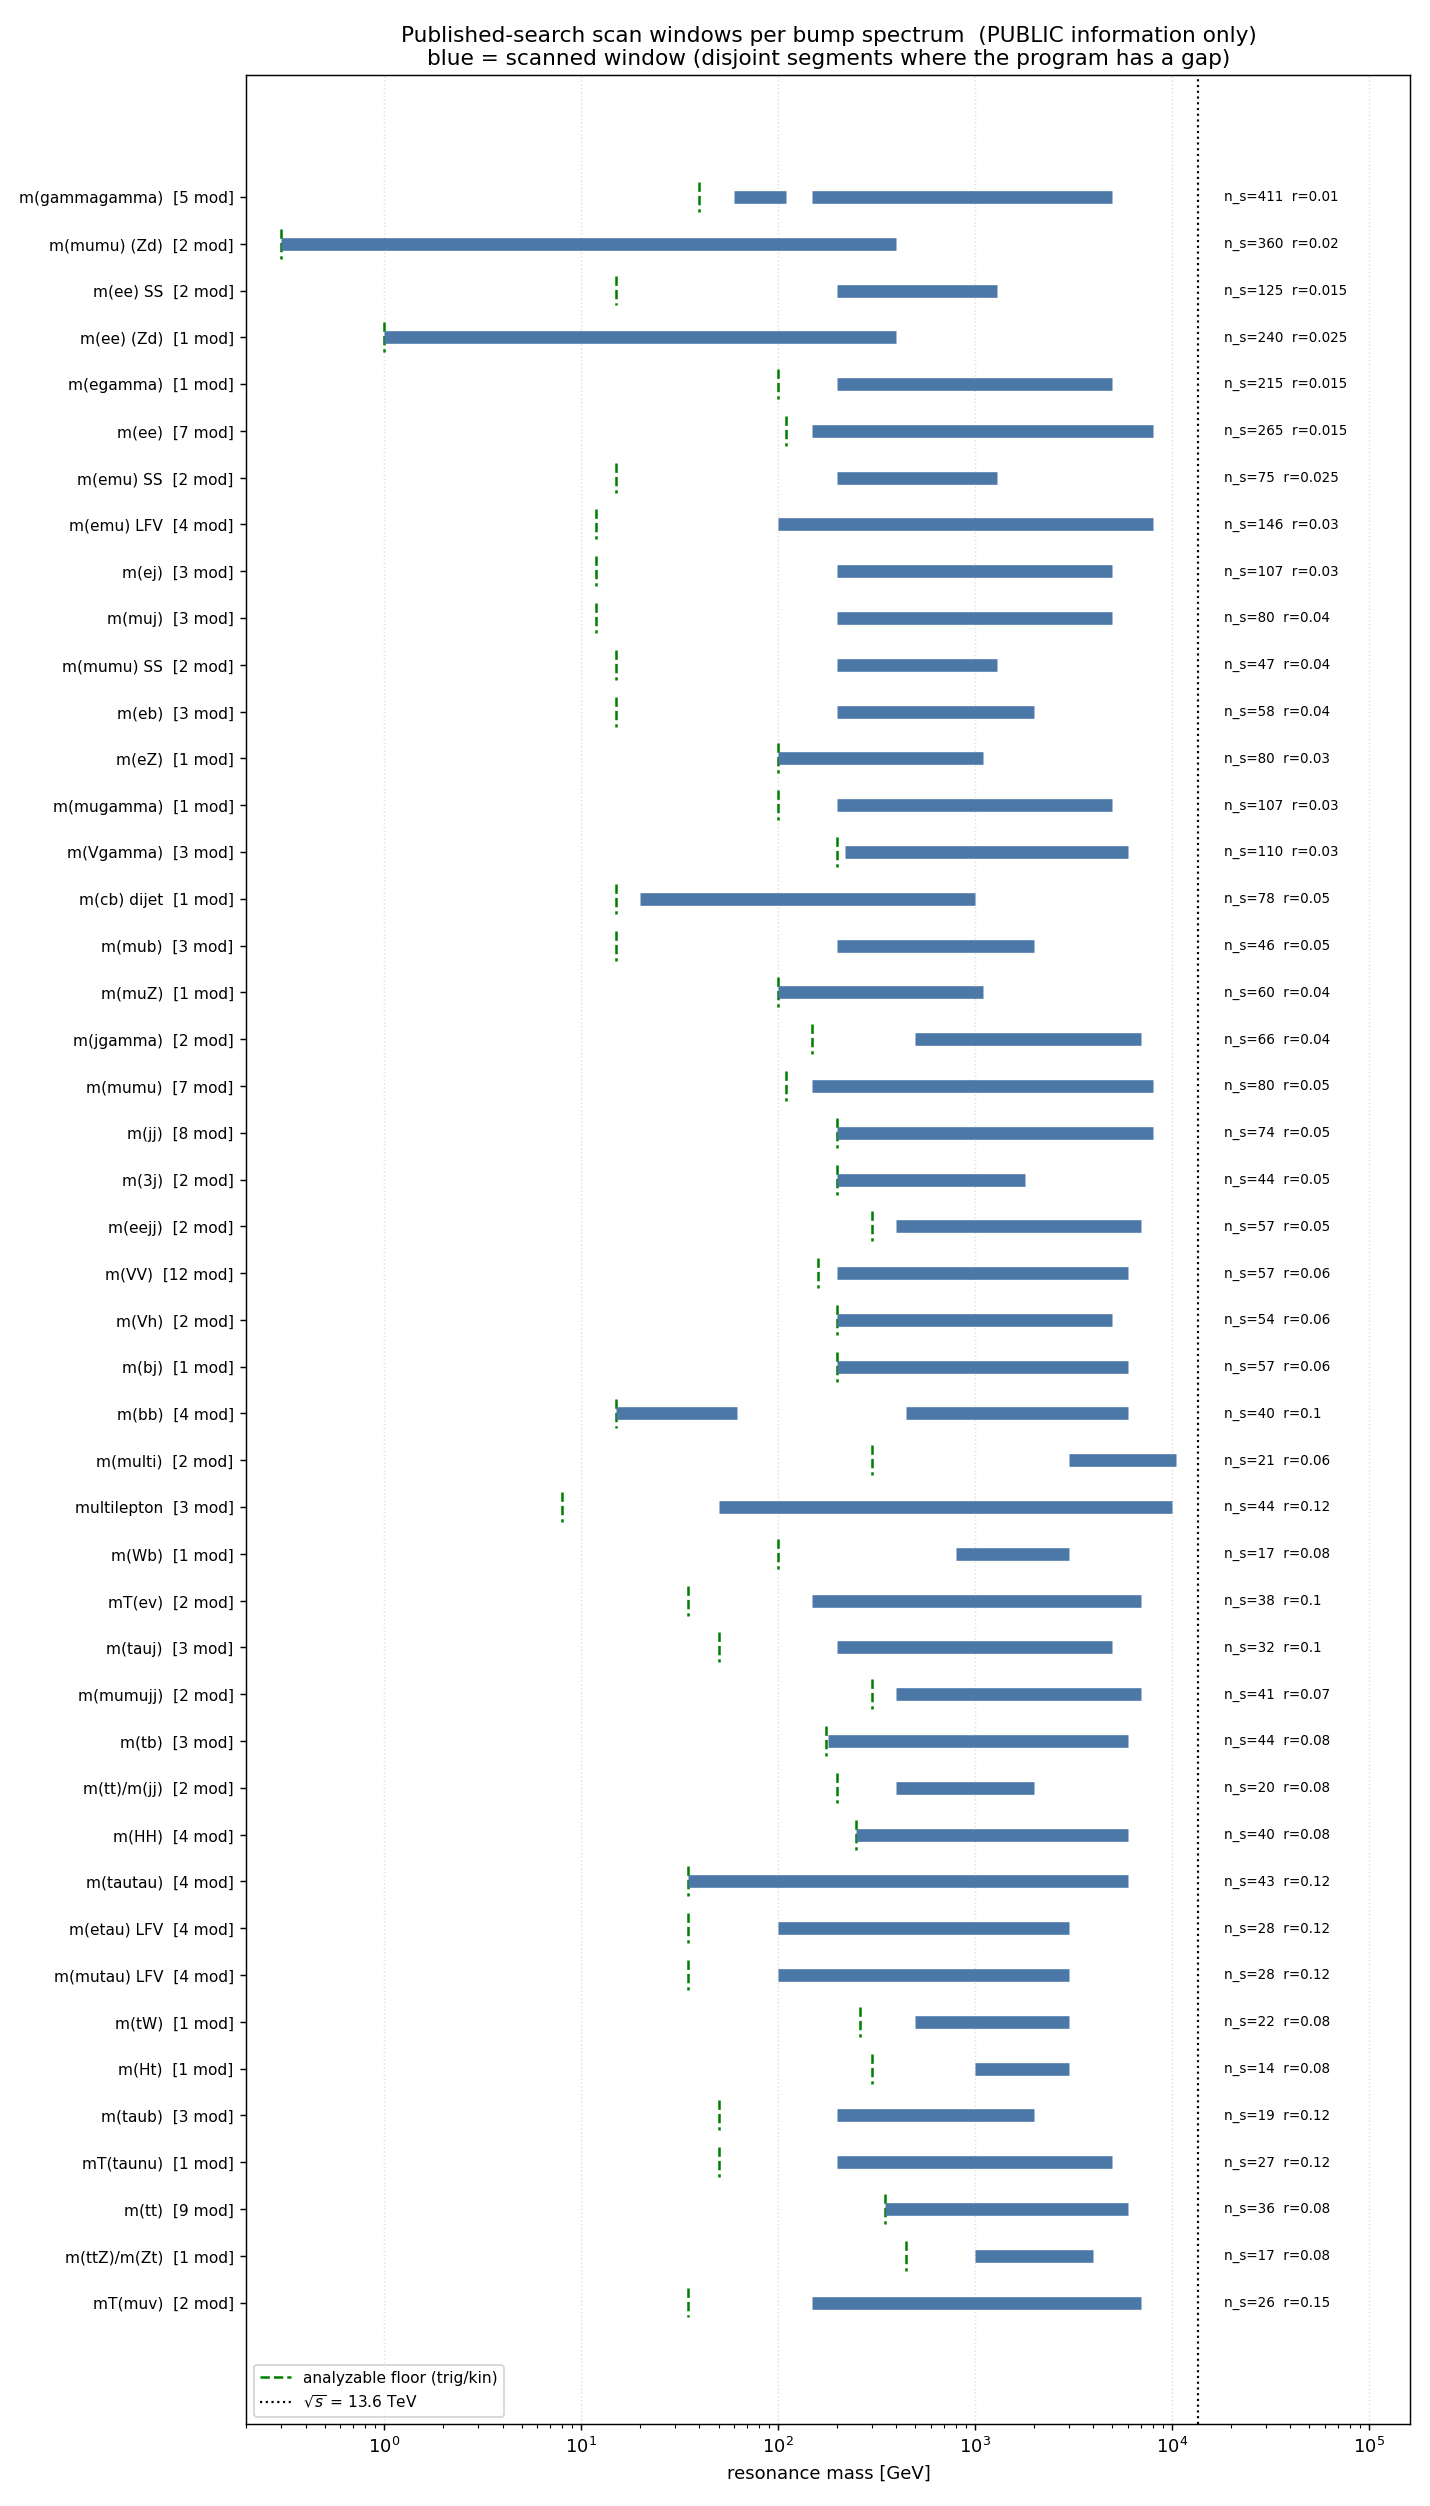
\includegraphics[width=0.95\textwidth,height=0.88\textheight,keepaspectratio]{scan_windows.png}
\caption{The scan windows of Table~\ref{tab:windows}, drawn per spectrum, with the analyzable floor
of each observable marked. Spectra scanned in disjoint segments ($m(\gamma\gamma)$, $m(bb)$) show
both.}
\label{fig:windows}
\end{figure}


\clearpage
\bibliographystyle{unsrtnat}
\bibliography{refs}

\end{document}
